\documentclass{article}

% Official NeurIPS 2026 style file, unmodified. Submission mode (no "final"):
% anonymous author block, line numbers on.
\usepackage[dblblindworkshop]{neurips_2026}
\workshoptitle{Machine Learning and the Physical Sciences}

% ML4PS 2026 requires this exact footer text. Set in the preamble; the .sty is not edited.
\makeatletter
\renewcommand{\@noticestring}{Submitted to the 9th Workshop on Machine Learning and the Physical Sciences (ML4PS 2026). Do not distribute.}
\makeatother

% Local build aid only: `pdflatex "\def\LOCALFONTCHECK{1}\documentclass{article}

% Official NeurIPS 2026 style file, unmodified. Submission mode (no "final"):
% anonymous author block, line numbers on.
\usepackage[dblblindworkshop]{neurips_2026}
\workshoptitle{Machine Learning and the Physical Sciences}

% ML4PS 2026 requires this exact footer text. Set in the preamble; the .sty is not edited.
\makeatletter
\renewcommand{\@noticestring}{Submitted to the 9th Workshop on Machine Learning and the Physical Sciences (ML4PS 2026). Do not distribute.}
\makeatother

% Local build aid only: `pdflatex "\def\LOCALFONTCHECK{1}\documentclass{article}

% Official NeurIPS 2026 style file, unmodified. Submission mode (no "final"):
% anonymous author block, line numbers on.
\usepackage[dblblindworkshop]{neurips_2026}
\workshoptitle{Machine Learning and the Physical Sciences}

% ML4PS 2026 requires this exact footer text. Set in the preamble; the .sty is not edited.
\makeatletter
\renewcommand{\@noticestring}{Submitted to the 9th Workshop on Machine Learning and the Physical Sciences (ML4PS 2026). Do not distribute.}
\makeatother

% Local build aid only: `pdflatex "\def\LOCALFONTCHECK{1}\documentclass{article}

% Official NeurIPS 2026 style file, unmodified. Submission mode (no "final"):
% anonymous author block, line numbers on.
\usepackage[dblblindworkshop]{neurips_2026}
\workshoptitle{Machine Learning and the Physical Sciences}

% ML4PS 2026 requires this exact footer text. Set in the preamble; the .sty is not edited.
\makeatletter
\renewcommand{\@noticestring}{Submitted to the 9th Workshop on Machine Learning and the Physical Sciences (ML4PS 2026). Do not distribute.}
\makeatother

% Local build aid only: `pdflatex "\def\LOCALFONTCHECK{1}\input{main.tex}"` swaps Times for
% Computer Modern on machines without the Times metrics. CM is wider, so a 4-page fit here is
% conservative. Inactive on Overleaf and in the submitted build.
\ifdefined\LOCALFONTCHECK
  \renewcommand{\rmdefault}{cmr}\renewcommand{\sfdefault}{cmss}\renewcommand{\ttdefault}{cmtt}
\fi

\usepackage[utf8]{inputenc}
\usepackage[T1]{fontenc}
\usepackage{hyperref}
\usepackage{url}
\usepackage{booktabs}
\usepackage{amsmath,amssymb}
\usepackage{microtype}
\usepackage{xcolor}
\usepackage{graphicx}

\newcommand{\Htan}{H^{S}}
\newcommand{\norm}[1]{\lVert #1 \rVert}

\title{Linear Probes on Curved Latent Spaces}

\author{%
  Anonymous Author(s)\\
  Affiliation\\
  \texttt{email}
}

\begin{document}

\maketitle

\begin{abstract}
Linear probes are commonly used to evaluate learned representations and infer physical quantities for objects without direct measurements. However, their global predictive performance does not reveal where individual predictions are locally reliable or how the geometry of the learned representation contributes to their errors. Here we identify a geometric source of local readout error. Although a linear probe is affine in the ambient space, its restriction to a curved embedding manifold has a nonzero intrinsic Hessian given by $\langle w_N,\mathrm{II}\rangle$, the manifold's bending contracted with the probe's normal component. We turn this classical identity into a per-object measurement on galaxy embeddings from five encoders, using a decoder-based estimate of the second fundamental form validated on a synthetic surface of known curvature. Comparing this probe-facing curvature with the intrinsic Hessian of the physical target, we find that their mismatch predicts local readout accuracy for magnitude and photometric redshift, robustly under cross-fitting and across encoders. A counterfactual intervention on a local second-order surrogate further shows that reversing the probe-facing bending reduces local accuracy at nearly every anchor, whereas randomly oriented bending of matched strength does not exhibit the same asymmetry. The resulting tensor mismatch provides a geometric diagnostic of local linear-readout reliability and helps identify which physical quantities exhibit geometry-associated variation in prediction accuracy.
\end{abstract}

\section{Introduction}

Linear probes evaluate learned representations by measuring how accurately targets can be recovered from frozen embeddings~\citep{alain2017probes}. Their global performance, however, does not reveal where individual predictions are reliable or how representation geometry contributes to their errors. This matters in physical science, where probes infer quantities without direct measurements. For galaxy images, linear probes predict catalogue quantities such as magnitude, redshift and stellar mass~\citep{smith2024astropt}, but offer no local reliability diagnostic. We show that an ambient affine probe inherits curvature from the embedding manifold in its normal direction. The mismatch between this probe-facing curvature and the target's intrinsic Hessian captures a local source of prediction error.

We contribute (i) a decoder-based pointwise estimate of the second fundamental form, validated on a synthetic surface of known curvature; (ii) the application of the classical identity $\operatorname{Hess}_M(w\cdot x)=\langle w_N,\mathrm{II}\rangle$ to a fitted probe, with a residual expansion identifying its second-order approximation error; and (iii) evidence from 86{,}471 galaxies and five encoders that curvature mismatch predicts local readout accuracy for magnitude and redshift, supported by an intervention on a local second-order surrogate with a matched random-direction control.


\section{Pointwise curvature from a decoder}
\label{sec:instr}

\paragraph{Data.} 86{,}471 galaxies from the AstroPT galaxy set~\citep{smith2024astropt} with catalogue labels ($r$-band magnitude, photometric redshift, smooth fraction, stellar mass), embedded by a supervised ImageNet-21k ViT-B/16 (``ViT-B'' below) and by four further encoders (Section~\ref{sec:real}); embeddings from the Platonic Universe release~\citep{duraphe2025platonic}. We unit-normalize embeddings (data on $S^{D-1}$; $D=768$ for ViT-B).

\paragraph{Instrument.} Let $F:\mathbb{R}^d\to\mathbb{R}^{D}$ be the decoder of a plain auto-encoder (three hidden layers of width 250, SiLU), fit on 80\% of rows; we evaluate curvature on held-out rows. With $J = DF(z)$, metric $g = J^{\top}J$, normal projector $P_N = I - Jg^{-1}J^{\top}$ and second fundamental form $\mathrm{II} = P_N D^2F(z)$, all by automatic differentiation (cf.~\citep{lee2023curvature,acosta2023extrinsic}) at points where $DF$ has full column rank $d$. We differentiate the projected decoder $F/\norm{F}$, whose image lies on the unit sphere, so that $\mathrm{II}$ splits exactly into the sphere's universal radial part and an in-sphere shape part (Eq.~\eqref{eq:split}; Appendix~E).

\paragraph{Validation.} On a synthetic in-sphere surface at $D=768$ with closed-form $\mathrm{II}$ (Appendix~E), the decoder's estimate matches the true trace of $\mathrm{II}$ in direction (cosine 0.999), magnitude (ratio 1.00) and rank across points (0.94).

\section{What a linear readout sees on a curved manifold}
\label{sec:theory}


\paragraph{Notation.}
Let $M\subset\mathbb{R}^D$ be a $d$-dimensional
smooth embedded manifold, $d<D$, with anchor
$x_0\in M$. Let $J$ be an orthonormal tangent
frame at $x_0$ and $u$ normal coordinates in
this frame, so that locally
$x(u)=x_0+Ju+\tfrac12\mathrm{II}(u,u)
+O(\|u\|^3)$~\citep{lee2018riemannian}, where $\mathrm{II}$ is the
normal-valued second fundamental form. In
the numerical estimates, $J=DF$ is the
decoder Jacobian, with metric $g=J^\top J$,
and tangent-projected coordinates are used.
A probe weight decomposes as $w=w_T+w_N$
into tangent and normal components. On the
unit sphere, $\mathrm{II}=\mathrm{II}^S-g\,x$
separates the in-sphere shape from the
universal radial bending, and $w_S$ is
the component of $w_N$ orthogonal to $x$.
Let $y$ be a smooth target on $M$ and
$\hat y=w\cdot x+b_0$ a global affine probe.
Tensor norms and inner products use
$\langle A,B\rangle_g
=g^{ia}g^{jb}A_{ij}B_{ab}$.

Three facts follow. First, although the
probe is affine in the ambient space, its
restriction to $M$ is generally nonlinear
in intrinsic coordinates:
\begin{equation}
(d\hat y)_J=J^\top w,\qquad
\operatorname{Hess}_M\hat y
=\langle w_N,\mathrm{II}\rangle=:K.
\label{eq:hess}
\end{equation}
We call $K$ the probe-facing curvature.
Second, on the unit sphere it splits into
an in-sphere shape term and a radial term:
\begin{equation}
K=
\underbrace{\langle w_S,\mathrm{II}^S
\rangle}_{K_S}
+
\underbrace{[-(\hat y-b_0)g]}_{K_{\mathrm{sph}}}.
\label{eq:split}
\end{equation}
Thus, even an ambient affine readout
inherits intrinsic curvature from the
geometry of the representation.

Third, consider an isotropic Gaussian
patch $u\sim N(0,s^2I_d)$ in the
orthonormal tangent frame. For sufficiently
smooth embedding and target functions,
with controlled higher derivatives, let
$\bar c=\mathbb E_{\mathrm{patch}}[y-\hat y]$
be the patch-mean residual,
$\delta=(dy-d\hat y)_J$ the differential
mismatch, and
$\Delta=\operatorname{Hess}_M y-K$
the Hessian mismatch. Then
\begin{equation}
\begin{aligned}
\mathbb E_{\mathrm{patch}}
[(y-\hat y)^2]
={}&\bar c^{\,2}
+s^2\|\delta\|^2\\
&+\tfrac12s^4\|\Delta\|_g^2
+O(s^4\|\delta\|)+O(s^6).
\end{aligned}
\label{eq:resid}
\end{equation}
The Hessian mismatch therefore determines
the quadratic residual's contribution
to centered local error under this model.
Its contribution is smaller than at
$K=0$ iff
$2\langle\operatorname{Hess}_M y,K
\rangle_g>\|K\|_g^2$: the probe-facing
curvature must bend toward the target's
curvature, without overshooting it.
With the sphere term fixed, the
corresponding condition for the shape
term is
$2\langle R,K_S\rangle_g>\|K_S\|_g^2$,
where
$R=\operatorname{Hess}_M y-K_{\mathrm{sph}}$.
Section~\ref{sec:real} tests this
relationship. Since the quadratic
contribution scales as $s^4$, our
empirical analysis controls for
variation in local neighborhood scale.

\section{Probe-facing curvature: bending toward the label helps, bending away hurts}
\label{sec:real}

Statistic: five-fold out-of-fold ridge probe~\citep{alain2017probes} at the pre-registered $\alpha=100$ from embedding to label; local $R^2$ inside each of 512 anchors' 2{,}048-neighbourhoods; rank-partial Spearman against local $R^2$ with Freedman--Lane $p$-values~\citep{freedman1983permutation}, controlling for log patch radius, local label variance and count and, stronger, log radius at five scales.

\begin{figure}[t]
\centering
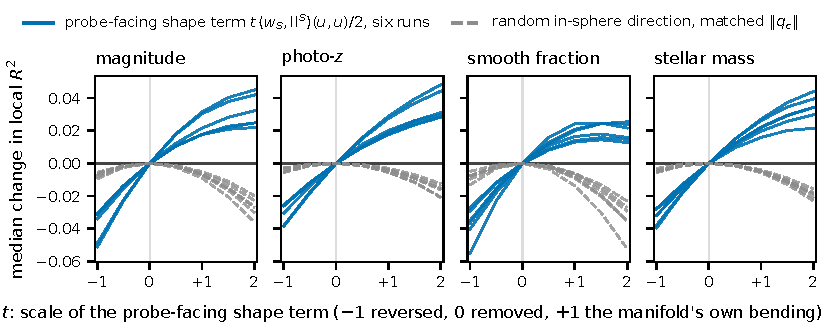
\includegraphics[width=\textwidth]{figures/fig1_intervention.pdf}
\caption{Bending toward the label helps, bending away hurts. At each of 512 anchors the readout's in-sphere shape quadratic $\tfrac t2\langle w_S,\mathrm{II}^S\rangle(u,u)$ is scaled by $t$ in a local second-order surrogate at a fixed manifold; lines are the median over anchors of the change in local $R^2$ relative to shape-flat ($t=0$). $t=1$ is the manifold's own bending seen from the readout's normal direction, $t=-1$ its reversal. Blue: the decoder's shape term, one line per run (five encoders at $d=16$, ViT-B also at $d=20$). Grey dashed: a random in-sphere normal direction with matched quadratic amplitude $\norm{q_c}$. Fractions of anchors helped and hurt, and sign tests on non-overlapping anchors, in Appendix~D.}
\label{fig:main}
\end{figure}

\paragraph{Galaxies.}
We estimate $\operatorname{Hess}_M y$ at each
anchor by fitting a least-squares quadratic
to the labels of its 2{,}048 neighbours in
tangent-projected coordinates
$u=g^{-1}J^\top(x-x_0)$. These decoder-based
Monge coordinates have vanishing Christoffel
symbols at the anchor, so the quadratic
coefficient estimates the covariant Hessian
in the small-neighbourhood limit. For
magnitude and redshift, the mismatch
$\|\Delta\|_g$ is negatively associated with
local $R^2$ ($-0.39$ to $-0.45$), while
alignment
$\cos_g(\operatorname{Hess}_M y,K)$
is positively associated with it
($+0.24$ to $+0.43$). These relationships
persist under cross-fitting (Appendix~B).
Smooth fraction exhibits weaker associations,
while stellar mass shows no significant
mismatch or alignment signal in this
experiment (Table~\ref{tab:real}; decoder
ablations, Appendix~A). Across five encoders, mismatch remains negatively associated with local accuracy for magnitude and redshift, while alignment is positive and significant for magnitude across all five and redshift across four (Appendix~C).

The shape term closely tracks the magnitude
of the total probe-facing curvature on
galaxies (rank correlation $0.96$--$0.99$),
but its association with local accuracy
varies across targets. This is consistent
with Eq.~\eqref{eq:resid}, where the shape
term's contribution to the quadratic
mismatch depends on both its magnitude and
its alignment with the remaining target
curvature. The sphere term is negatively
associated with local accuracy for all four
targets in the main ViT-B experiment,
although its association is sensitive to
probe regularization for some targets
(Appendix~E). Applying the same local
quadratic regression to the probe predictions
provides a decoder-independent estimate of
$K$, with median tensor cosine
$0.55$--$0.65$ relative to the
decoder-based estimate.

\paragraph{Relation to prior work.}
The identity in Eq.~\eqref{eq:hess} is
classical~\citep{milnor1963morse,chern1957total};
related work derives a curvature-dependent
normal weight for least-squares regression
on hypersurfaces~\citep{liu2023linear}
and documents the effects of curved
representations on linear
decoding~\citep{jurewicz2024irrational}.
Other approaches study manifold
capacity~\citep{chung2016linear,slatton2026linear},
representation flattening~\citep{psenka2024flattening},
curvature regularization~\citep{ma2023curvature},
latent geometry~\citep{kaufman2023latent},
local-regression bias~\citep{cheng2013local},
and geometric indicators of
generalization~\citep{chou2026diagnosing}.
Our contribution is to estimate the
pointwise probe-facing curvature tensor
on a learned manifold, compare it with
the target's intrinsic Hessian, and test
its contribution to local readout accuracy
through a controlled second-order intervention.

\paragraph{Bending toward helps, bending away hurts.}
To isolate the contribution of probe-facing
shape curvature, we intervene on the
in-sphere quadratic term of a local
second-order surrogate while keeping the
manifold, tangent readout, and sphere term
fixed. Each anchor's 2{,}048 neighbours
are scored by
$\hat y_t(u)=c+a^\top u+
\tfrac12K_{\mathrm{sph}}(u,u)+
\tfrac t2K_S(u,u)$,
where $a$ is the probe's tangent
differential, $K_S$ is estimated from the
decoder, and $c$ is refit for each $t$.
Here $t=1$ retains the estimated shape
quadratic of the original readout,
$t=-1$ reverses its sign, and $t=0$
removes it.

Under the isotropic Gaussian quadratic
model, $t=1$ improves upon $t=0$ iff
$2\langle R,K_S\rangle_g>\|K_S\|_g^2$.
On the actual neighbours, let $r_0$ be
the centred shape-flat residual and
$q_c$ the centred quadratic contribution
$\tfrac12K_S(u_i,u_i)$. After refitting
the intercept, the exact finite-sample
criterion is
$2\langle r_0,q_c\rangle>\|q_c\|^2$,
with optimum
$t^*=\langle r_0,q_c\rangle/\|q_c\|^2$
(Appendix~D).

Across five encoders and all four labels
(Figure~\ref{fig:main}), $t=1$ improves
local $R^2$ relative to the shape-flat
surrogate at 79--99\% of anchors, while
$t=-1$ reduces it at 97--100\%.
A random in-sphere normal direction with
matched centred quadratic amplitude shows
no comparable directional asymmetry and
is typically harmful under either sign
($t=1$ improves upon shape-flat at
22--36\% of anchors; Appendix~D).

Thus, the probe-selected shape quadratic
is locally error-reducing within the
second-order surrogate. Under the quadratic
Gaussian model, this is the signature of
bending toward the target's remaining
intrinsic curvature. This within-anchor
comparison differs from the cross-anchor
associations in Table~\ref{tab:real}
and can hold even where the latter show
no significant signal, as for stellar mass.
The optimum $t^*$ lies between 1.5 and
3.6 across runs, indicating that further
amplification of the shape term reduces
local surrogate error. 

\section{Discussion}

Our results identify a geometric source of local linear-probe error: the mismatch $\Delta=\operatorname{Hess}_M y-\langle w_N,\mathrm{II}\rangle$ between the target's intrinsic Hessian and the curvature induced by the probe. We estimate this mismatch using a decoder-based second fundamental form, validated on a synthetic surface and showing moderate agreement with a decoder-independent estimate on galaxy embeddings. Across five encoders, mismatch tracks local accuracy for magnitude and redshift, with weaker evidence for smooth fraction. A counterfactual intervention on the local second-order surrogate shows that the probe-selected shape term reduces error at most anchors, while reversing it generally increases error. Thus, manifold curvature can help rather than hinder linear decoding when it bends toward the target's curvature.

The mismatch can be estimated from labelled neighbours without knowing an object's target value, providing a local diagnostic of predictions that may warrant further scrutiny. It is not yet a calibrated per-object uncertainty estimate. For stellar mass, mismatch does not consistently track local accuracy despite the beneficial shape contribution, showing that a locally useful geometric effect need not explain variation in overall readout accuracy.

\emph{Limitations.}
We study one galaxy sample, four targets and five encoders. The label Hessian is estimated from finite neighbourhoods; its norm is reliably ranked (split-half $\rho=0.91$--$0.94$), but its direction is only moderately recovered (tensor cosine $0.19$--$0.35$). The synthetic surface does not independently corroborate the alignment association because its target has insufficient intrinsic curvature. The intervention modifies a local surrogate, not the encoder or manifold. Mismatch and alignment are the primary hypotheses; other analyses are exploratory. Overlapping neighbourhoods introduce anchor dependence that may affect permutation-test validity.

\bibliographystyle{unsrtnat}
{\small
\bibliography{references}
}

\appendix
% BEGIN APPENDIX AUTOGEN
\section*{Appendix A: decoder ablations}
Table~\ref{tab:ablate} repeats the four quantities of Tables~\ref{tab:real} and~\ref{tab:meancurv} at $d=16$ under the multi-scale density control for two further decoder initialisation seeds and for a decoder of width $400^3$ instead of $250^3$ (all fits reach variance explained 0.952). Every significant sign of the main table is retained.
\begin{table}[h]
\centering\footnotesize\setlength{\tabcolsep}{4pt}
\begin{tabular}{llcccc}
\toprule
label & quantity & seed 0 & seed 1 & seed 2 & $400^3$ \\
\midrule
mag\_r & shape & $+0.12$ & $+0.05^{*}$ & $+0.12$ & $+0.05^{*}$ \\
 & sphere & $-0.26$ & $-0.26$ & $-0.27$ & $-0.26$ \\
 & mismatch & $-0.39$ & $-0.35$ & $-0.34$ & $-0.34$ \\
 & alignment & $+0.35$ & $+0.31$ & $+0.37$ & $+0.41$ \\
\addlinespace[2pt]
photo\_z & shape & $-0.06^{*}$ & $-0.09^{*}$ & $-0.09$ & $-0.06^{*}$ \\
 & sphere & $-0.33$ & $-0.35$ & $-0.34$ & $-0.35$ \\
 & mismatch & $-0.45$ & $-0.43$ & $-0.42$ & $-0.41$ \\
 & alignment & $+0.26$ & $+0.24$ & $+0.25$ & $+0.25$ \\
\addlinespace[2pt]
smooth\_fraction & shape & $+0.07^{*}$ & $+0.20$ & $+0.15$ & $+0.10$ \\
 & sphere & $-0.13$ & $-0.15$ & $-0.14$ & $-0.11$ \\
 & mismatch & $-0.09^{*}$ & $-0.05^{*}$ & $-0.08^{*}$ & $-0.07^{*}$ \\
 & alignment & $+0.19$ & $+0.14$ & $+0.09$ & $+0.10$ \\
\addlinespace[2pt]
stellar\_mass & shape & $+0.00^{*}$ & $-0.06^{*}$ & $+0.05^{*}$ & $+0.09$ \\
 & sphere & $-0.35$ & $-0.35$ & $-0.35$ & $-0.35$ \\
 & mismatch & $-0.04^{*}$ & $+0.03^{*}$ & $+0.02^{*}$ & $+0.03^{*}$ \\
 & alignment & $+0.01^{*}$ & $-0.02^{*}$ & $+0.03^{*}$ & $-0.02^{*}$ \\
\addlinespace[2pt]
\bottomrule
\end{tabular}
\caption{Decoder ablations, $d=16$, 512 anchors, multi-scale density control. $^{*}$ not significant at 0.05.}
\label{tab:ablate}
\end{table}
\section*{Appendix B: sensitivity of the mismatch and sphere columns}
Cross-fitting: each 2{,}048-patch is split at random into halves; $\operatorname{Hess}_M y$ is fitted on one half and local $R^2$ scored on the other (both directions shown), so the Hessian estimate and the outcome share no rows. The split-half cosine between the two Hessian estimates is the reliability of the estimate. Weak ridge: the probe refit at $\alpha=1$ instead of 100 (global out-of-sample $R^2$ rises by 0.10 to 0.15), which substantially reduces the shrinkage of extreme predictions; the sphere term is recomputed from that probe.
\begin{table}[h]
\centering\footnotesize\setlength{\tabcolsep}{3.5pt}
\begin{tabular}{llcccccc}
\toprule
 & & \multicolumn{2}{c}{mismatch, cross-fit} & \multicolumn{2}{c}{alignment, cross-fit} & Hess.\ split cos & sphere, $\alpha=1$ \\
label & $d$ & fit A/score B & fit B/score A & fit A/score B & fit B/score A & p50 & (main: $\alpha=100$) \\
\midrule
mag\_r & 16 & $-0.38$ & $-0.34$ & $+0.33$ & $+0.31$ & +0.35 & $-0.21$ ($-0.26$) \\
mag\_r & 20 & $-0.43$ & $-0.40$ & $+0.39$ & $+0.37$ & +0.24 & $-0.22$ ($-0.26$) \\
photo\_z & 16 & $-0.42$ & $-0.36$ & $+0.23$ & $+0.20$ & +0.32 & $+0.05^{*}$ ($-0.33$) \\
photo\_z & 20 & $-0.42$ & $-0.42$ & $+0.22$ & $+0.22$ & +0.20 & $+0.03^{*}$ ($-0.36$) \\
smooth\_fraction & 16 & $-0.10$ & $-0.17$ & $+0.17$ & $+0.19$ & +0.33 & $-0.12$ ($-0.13$) \\
smooth\_fraction & 20 & $-0.15$ & $-0.21$ & $+0.05^{*}$ & $+0.03^{*}$ & +0.23 & $-0.13$ ($-0.15$) \\
stellar\_mass & 16 & $+0.01^{*}$ & $-0.04^{*}$ & $-0.03^{*}$ & $+0.06^{*}$ & +0.31 & $-0.02^{*}$ ($-0.35$) \\
stellar\_mass & 20 & $-0.06^{*}$ & $-0.07^{*}$ & $+0.01^{*}$ & $-0.00^{*}$ & +0.19 & $-0.02^{*}$ ($-0.35$) \\
\bottomrule
\end{tabular}
\caption{Cross-fitted mismatch and alignment partials (multi-scale control), split-half reliability of the label Hessian, and the sphere-term partial under a weak-ridge probe.}
\label{tab:sens}
\end{table}

\section*{Appendix C: Main and cross-encoder results}

\paragraph{Main results.}
Table~\ref{tab:real} reports the associations
between geometric mismatch, alignment and local
readout accuracy for ViT-B at $d=16$ and $d=20$.
Results use 512 anchors, $k=2{,}048$ neighbours
and the multi-scale density control.

\begin{table}[h]
\centering
\footnotesize
\setlength{\tabcolsep}{3.4pt}
\begin{tabular}{lcccc}
\toprule
 & \multicolumn{2}{c}{mismatch $\norm{\Delta}_g$}
 & \multicolumn{2}{c}{alignment $\cos_g(\operatorname{Hess}_M y, K)$} \\
label & $d{=}16$ & $d{=}20$ & $d{=}16$ & $d{=}20$ \\
\midrule
mag\_r & $-0.39$ & $-0.40$ & $+0.35$ & $+0.43$ \\
photo\_z & $-0.45$ & $-0.44$ & $+0.26$ & $+0.24$ \\
smooth\_fraction & $-0.09^{*}$ & $-0.17$ & $+0.19$ & $+0.07^{*}$ \\
stellar\_mass & $-0.04^{*}$ & $-0.09^{*}$ & $+0.01^{*}$ & $+0.02^{*}$ \\
\bottomrule
\end{tabular}
\caption{ViT-B: rank-partial Spearman correlations
with local $R^2$ under the multi-scale density
control. $^{*}$ Not significant at 0.05.
Shape, sphere and mean-curvature results
are reported in Appendix~E.}
\label{tab:real}
\end{table}

\paragraph{Across encoders.}
We repeat the geometric diagnostic at $d=16$
on the same 86{,}471 galaxies using four further
encoders from the Platonic Universe release:
DINOv3 ViT-B/16, CLIP ViT-B, ConvNeXt-B and
ViT-L (widths 768, 512, 1{,}024 and 1{,}024;
all unit-normalized).
A decoder of the same architecture and training
protocol is fitted per encoder (seed 0;
variance explained 0.966, 0.985, 0.965 and
0.968, respectively). All analyses use
512 anchors, $k=2{,}048$ and the multi-scale
density control.

For magnitude and redshift, mismatch is
negatively associated with local $R^2$
across all five encoders ($-0.32$ to $-0.61$;
cross-fitted $-0.28$ to $-0.62$).
Alignment is positive and significant for
magnitude across all five ($+0.13$ to $+0.53$)
and for redshift across four.
Shape-term associations vary by encoder and
target, while smooth fraction shows less
consistent mismatch and alignment signals.
For stellar mass, alignment is nonsignificant
across encoders and mismatch significant in
only one main comparison. Thus, the
cross-anchor mismatch association varies by
target, even where the shape term improves
the local surrogate.

Table~\ref{tab:xenc} reports the full
cross-encoder results, including global
out-of-sample probe $R^2$ in the first row
for each label. Table~\ref{tab:xencx}
reports cross-fitted mismatch and alignment
associations and split-half reliability of
the estimated label Hessian.

\begin{table}[h]
\centering
\footnotesize
\setlength{\tabcolsep}{4pt}
\begin{tabular}{llccccc}
\toprule
label & quantity & ViT-B & DINOv3 & CLIP-B & ConvNeXt-B & ViT-L \\
\midrule
mag\_r & global $R^2$ & 0.52 & 0.57 & 0.50 & 0.52 & 0.52 \\
 & shape & $+0.12$ & $-0.11$ & $+0.16$ & $+0.16$ & $-0.21$ \\
 & sphere & $-0.26$ & $-0.23$ & $-0.40$ & $-0.24$ & $-0.08^{*}$ \\
 & mismatch & $-0.39$ & $-0.57$ & $-0.34$ & $-0.32$ & $-0.44$ \\
 & alignment & $+0.35$ & $+0.53$ & $+0.32$ & $+0.21$ & $+0.13$ \\
\addlinespace[2pt]
photo\_z & global $R^2$ & 0.51 & 0.56 & 0.49 & 0.49 & 0.51 \\
 & shape & $-0.06^{*}$ & $-0.05^{*}$ & $-0.17$ & $+0.29$ & $-0.16$ \\
 & sphere & $-0.33$ & $-0.21$ & $-0.29$ & $-0.46$ & $-0.44$ \\
 & mismatch & $-0.45$ & $-0.61$ & $-0.45$ & $-0.48$ & $-0.46$ \\
 & alignment & $+0.26$ & $+0.33$ & $+0.06^{*}$ & $+0.22$ & $+0.14$ \\
\addlinespace[2pt]
smooth\_fraction & global $R^2$ & 0.53 & 0.59 & 0.49 & 0.56 & 0.55 \\
 & shape & $+0.07^{*}$ & $-0.08^{*}$ & $+0.20$ & $+0.24$ & $+0.06^{*}$ \\
 & sphere & $-0.13$ & $-0.06^{*}$ & $+0.05^{*}$ & $-0.15$ & $-0.11$ \\
 & mismatch & $-0.09^{*}$ & $-0.33$ & $-0.25$ & $-0.20$ & $-0.01^{*}$ \\
 & alignment & $+0.19$ & $-0.02^{*}$ & $+0.24$ & $+0.04^{*}$ & $+0.14$ \\
\addlinespace[2pt]
stellar\_mass & global $R^2$ & 0.48 & 0.54 & 0.50 & 0.49 & 0.49 \\
 & shape & $+0.00^{*}$ & $-0.15$ & $-0.10$ & $-0.11$ & $-0.13$ \\
 & sphere & $-0.35$ & $-0.26$ & $-0.38$ & $-0.40$ & $-0.38$ \\
 & mismatch & $-0.04^{*}$ & $+0.03^{*}$ & $-0.12$ & $-0.06^{*}$ & $-0.02^{*}$ \\
 & alignment & $+0.01^{*}$ & $-0.05^{*}$ & $-0.01^{*}$ & $+0.07^{*}$ & $-0.03^{*}$ \\
\addlinespace[2pt]
\bottomrule
\end{tabular}
\caption{Cross-encoder results at $d=16$:
global probe $R^2$ and rank-partial Spearman
correlations with local $R^2$ under the
multi-scale density control.
$^{*}$ Not significant at 0.05.}
\label{tab:xenc}
\end{table}

\begin{table}[h]
\centering
\footnotesize
\setlength{\tabcolsep}{3.5pt}
\begin{tabular}{llccccc}
\toprule
 & & \multicolumn{2}{c}{mismatch, cross-fit}
 & \multicolumn{2}{c}{alignment, cross-fit}
 & Hess.\ split cos \\
encoder & label & fit A/score B & fit B/score A
& fit A/score B & fit B/score A & p50 \\
\midrule
\addlinespace[2pt]
DINOv3 & mag\_r & $-0.60$ & $-0.62$ & $+0.50$ & $+0.50$ & +0.35 \\
 & photo\_z & $-0.56$ & $-0.59$ & $+0.28$ & $+0.27$ & +0.24 \\
 & smooth\_fraction & $-0.32$ & $-0.29$ & $-0.03^{*}$ & $-0.02^{*}$ & +0.31 \\
 & stellar\_mass & $+0.03^{*}$ & $+0.02^{*}$ & $-0.03^{*}$ & $-0.07^{*}$ & +0.22 \\
\addlinespace[2pt]
CLIP-B & mag\_r & $-0.28$ & $-0.35$ & $+0.28$ & $+0.29$ & +0.31 \\
 & photo\_z & $-0.41$ & $-0.40$ & $+0.08^{*}$ & $+0.06^{*}$ & +0.25 \\
 & smooth\_fraction & $-0.22$ & $-0.24$ & $+0.15$ & $+0.20$ & +0.28 \\
 & stellar\_mass & $-0.14$ & $-0.13$ & $-0.04^{*}$ & $+0.01^{*}$ & +0.19 \\
\addlinespace[2pt]
ConvNeXt-B & mag\_r & $-0.36$ & $-0.34$ & $+0.19$ & $+0.21$ & +0.29 \\
 & photo\_z & $-0.46$ & $-0.45$ & $+0.18$ & $+0.19$ & +0.30 \\
 & smooth\_fraction & $-0.15$ & $-0.19$ & $-0.02^{*}$ & $+0.03^{*}$ & +0.32 \\
 & stellar\_mass & $-0.05^{*}$ & $-0.01^{*}$ & $+0.14$ & $-0.03^{*}$ & +0.29 \\
\addlinespace[2pt]
ViT-L & mag\_r & $-0.46$ & $-0.49$ & $+0.09^{*}$ & $+0.15$ & +0.30 \\
 & photo\_z & $-0.44$ & $-0.42$ & $+0.09^{*}$ & $+0.13$ & +0.24 \\
 & smooth\_fraction & $-0.03^{*}$ & $-0.04^{*}$ & $+0.11$ & $+0.07^{*}$ & +0.30 \\
 & stellar\_mass & $-0.06^{*}$ & $+0.01^{*}$ & $-0.04^{*}$ & $-0.03^{*}$ & +0.21 \\
\addlinespace[2pt]
\bottomrule
\end{tabular}
\caption{Cross-fitted mismatch and alignment
partials under the multi-scale density
control, with median split-half tensor
cosine for the estimated label Hessian.
$^{*}$ Not significant at 0.05.}
\label{tab:xencx}
\end{table}
\section*{Appendix D: intervening on the readout's normal component}
The partials of Table~\ref{tab:real} compare anchors with one another and cannot say whether reversing the probe-facing shape term hurts relative to removing it, since no anchor is flat. Here we score a counterfactual local second-order surrogate of the readout at a fixed manifold. At each anchor the fitted ridge weight is split into tangent, radial and in-sphere normal parts $w = w_T + w_{\mathrm{rad}} + w_S$; we score the anchor's 2{,}048 neighbours by the data-side tangent-plus-sphere readout $(w_T + w_{\mathrm{rad}})\cdot x$ plus $t\,q$ with the local intercept refit, where $q = \tfrac12\langle w_S,\mathrm{II}^S\rangle(u,u)$ is the decoder's in-sphere second-order term in the anchor's chart coordinates: $t=1$ is the manifold's bending as seen in the readout's normal direction, $t=-1$ its sign reversal, $t=0$ shape-flat (the sphere term $-(w\!\cdot\!\hat x)g$ is kept in the base). Because the intercept is refit for every $t$, the local sum of squares is exactly $\mathrm{SSE}(t) = \norm{r_0 - t\,q_c}^2$ with $r_0$ the centred residual of the shape-flat predictor and $q_c = q - \bar q\mathbf 1$ the centred quadratic on the anchor's neighbours; hence $t^{*} = \langle r_0,q_c\rangle/\norm{q_c}^2$ and $t=1$ beats shape-flat iff $2\langle r_0,q_c\rangle > \norm{q_c}^2$. This is the finite-sample counterpart of the tensor-level condition $2\langle R,K_S\rangle_g > \norm{K_S}_g^2$ of Section~\ref{sec:theory}, not the same quantity: the tensor version needs the estimated label Hessian, the empirical one does not. Columns: fraction of anchors where $t=1$ beats shape-flat (help) and where $t=-1$ is worse than shape-flat (hurt), the median change in local $R^2$ at $t=\pm1$, the median $t^{*}$; then the same for a random in-sphere normal direction $v$ whose quadratic is rescaled to the same centred amplitude on the actual neighbours, $\norm{q_{v,c}} = \norm{q_c}$ (matching $\norm{v}$ to $\norm{w_S}$ instead leaves the contracted tensor at a fraction of the fitted one, since $\mathrm{II}^S$ spans at most $d(d+1)/2$ of the $\sim 750$ normal directions; matching $\norm{\langle v,\mathrm{II}^S\rangle}_g$ gives the same picture; Supplement 12). The anchors' neighbourhoods overlap (each point lies in about twelve of them), so the fractions are not counts of independent trials; a maximal set of anchors whose pairwise overlap is at most 5\% of $k$ has 19--21 members per run, on which $t=1$ beats shape-flat at 81--100\% (one-sided sign test $p \le 4\times 10^{-3}$ in every cell) and $t=-1$ is worse at 95--100\% ($p \le 3\times 10^{-5}$).
\begin{table}[h]
\centering\footnotesize\setlength{\tabcolsep}{3pt}
\begin{tabular}{llccccc|cccc}
\toprule
 & & \multicolumn{5}{c|}{decoder in-sphere shape term} & \multicolumn{4}{c}{random orientation, matched $\norm{q_c}$} \\
run & label & help & hurt & $\Delta R^2(+1)$ & $\Delta R^2(-1)$ & $t^{*}$ & help & hurt & $\Delta R^2(+1)$ & $\Delta R^2(-1)$ \\
\midrule
ViT-B, $d=16$ & mag\_r & 0.97 & 1.00 & $+0.030$ & $-0.051$ & 2.3 & 0.26 & 0.80 & $-0.009$ & $-0.009$ \\
 & photo\_z & 0.99 & 0.99 & $+0.028$ & $-0.038$ & 3.0 & 0.33 & 0.68 & $-0.005$ & $-0.006$ \\
 & smooth\_fraction & 0.90 & 1.00 & $+0.021$ & $-0.040$ & 1.7 & 0.24 & 0.78 & $-0.008$ & $-0.010$ \\
 & stellar\_mass & 0.96 & 0.99 & $+0.026$ & $-0.040$ & 2.6 & 0.29 & 0.70 & $-0.006$ & $-0.006$ \\
\addlinespace[2pt]
ViT-B, $d=20$ & mag\_r & 0.99 & 1.00 & $+0.031$ & $-0.049$ & 2.6 & 0.24 & 0.78 & $-0.007$ & $-0.008$ \\
 & photo\_z & 0.99 & 1.00 & $+0.029$ & $-0.038$ & 3.6 & 0.36 & 0.71 & $-0.004$ & $-0.005$ \\
 & smooth\_fraction & 0.90 & 1.00 & $+0.020$ & $-0.035$ & 1.9 & 0.22 & 0.77 & $-0.007$ & $-0.008$ \\
 & stellar\_mass & 0.97 & 1.00 & $+0.027$ & $-0.038$ & 3.1 & 0.32 & 0.72 & $-0.005$ & $-0.005$ \\
\addlinespace[2pt]
DINOv3, $d=16$ & mag\_r & 0.92 & 0.99 & $+0.018$ & $-0.031$ & 2.0 & 0.29 & 0.71 & $-0.007$ & $-0.006$ \\
 & photo\_z & 0.96 & 0.99 & $+0.020$ & $-0.030$ & 2.6 & 0.29 & 0.71 & $-0.006$ & $-0.004$ \\
 & smooth\_fraction & 0.93 & 1.00 & $+0.024$ & $-0.055$ & 1.5 & 0.22 & 0.78 & $-0.014$ & $-0.013$ \\
 & stellar\_mass & 0.95 & 1.00 & $+0.016$ & $-0.028$ & 2.1 & 0.26 & 0.74 & $-0.005$ & $-0.005$ \\
\addlinespace[2pt]
CLIP-B, $d=16$ & mag\_r & 0.95 & 0.99 & $+0.018$ & $-0.031$ & 2.2 & 0.30 & 0.68 & $-0.006$ & $-0.005$ \\
 & photo\_z & 0.99 & 1.00 & $+0.019$ & $-0.026$ & 3.4 & 0.36 & 0.64 & $-0.003$ & $-0.003$ \\
 & smooth\_fraction & 0.92 & 0.99 & $+0.014$ & $-0.027$ & 1.7 & 0.25 & 0.69 & $-0.006$ & $-0.005$ \\
 & stellar\_mass & 0.97 & 1.00 & $+0.020$ & $-0.028$ & 2.8 & 0.35 & 0.68 & $-0.004$ & $-0.005$ \\
\addlinespace[2pt]
ConvNeXt-B, $d=16$ & mag\_r & 0.92 & 1.00 & $+0.018$ & $-0.031$ & 2.0 & 0.26 & 0.73 & $-0.007$ & $-0.007$ \\
 & photo\_z & 0.99 & 1.00 & $+0.018$ & $-0.026$ & 2.9 & 0.28 & 0.64 & $-0.004$ & $-0.003$ \\
 & smooth\_fraction & 0.88 & 0.98 & $+0.016$ & $-0.036$ & 1.6 & 0.23 & 0.75 & $-0.009$ & $-0.008$ \\
 & stellar\_mass & 0.99 & 1.00 & $+0.022$ & $-0.032$ & 3.1 & 0.29 & 0.65 & $-0.005$ & $-0.003$ \\
\addlinespace[2pt]
ViT-L, $d=16$ & mag\_r & 0.96 & 0.99 & $+0.022$ & $-0.034$ & 2.6 & 0.32 & 0.74 & $-0.005$ & $-0.006$ \\
 & photo\_z & 0.97 & 0.99 & $+0.018$ & $-0.025$ & 3.2 & 0.34 & 0.67 & $-0.004$ & $-0.003$ \\
 & smooth\_fraction & 0.79 & 0.97 & $+0.013$ & $-0.029$ & 1.6 & 0.25 & 0.77 & $-0.006$ & $-0.008$ \\
 & stellar\_mass & 0.98 & 1.00 & $+0.022$ & $-0.032$ & 2.9 & 0.30 & 0.67 & $-0.004$ & $-0.004$ \\
\addlinespace[2pt]
\bottomrule
\end{tabular}
\caption{Counterfactual scaling of the in-sphere shape term in a local second-order surrogate of the readout, 512 anchors per run. The manifold's bending as seen in the readout's normal direction helps at a large majority of anchors, its sign reversal hurts at nearly every anchor, a random orientation of the same centred quadratic amplitude shows no such asymmetry and is typically harmful under either sign; $t^{*}>1$ throughout, consistent with the globally ridge-regularized probe under-using a locally beneficial term.}
\label{tab:cf}
\end{table}
% END APPENDIX AUTOGEN

% Appendix E is hand-written (not generated); numbers are the same record-verified values that stood in the main text until 2026-09-18.
\section*{Appendix E: the shape and sphere terms, and mean curvature}
\label{app:meancurv}
The mean-curvature vector of the decoder surface is $H = \operatorname{tr}_g \mathrm{II}$ (unnormalized trace; some authors divide by $d$). Alongside Eq.~\eqref{eq:hess}, $\Delta_M (w\!\cdot\! x) = \langle w, H\rangle$: the Laplacian of a linear readout sees only the trace of $\mathrm{II}$, its Hessian the whole tensor, so $\norm{H}$ need not track $\langle w_N,\mathrm{II}\rangle$. On the unit sphere the Euclidean mean-curvature vector of every $d$-submanifold has the universal radial component $-d\,\hat x$, which says nothing about shape; differentiating the projected decoder $F/\norm{F}$ splits $H = -d\,\hat x + \Htan$ exactly (radial part $-d$ to $10^{-14}$), and $\Htan$ is the non-radial mean-curvature component used below.

\emph{Validation surface.} At $D=768$ the in-sphere surface $G(z) = Q\,\mathrm{normalize}([\phi(z);\,0.8\,h(z);\,0\ldots])$ ($\phi$ inverse stereographic $\mathbb{R}^{16}\to S^{16}$, $h$ four Gaussian bumps, $Q$ a rotation) has closed-form curvature; the decoder's $\Htan$ gives rank 0.94 against the true $\norm{\Htan}$, direction cosine 0.999, magnitude ratio 1.00. Resampling this surface with weight $\norm{\Htan}^\gamma$ (Figure~\ref{fig:meancurv}a) moves the density-controlled $\norm{\Htan}$ partial against local $R^2$ from $-0.29$ to $+0.26$, while $\norm{\langle w_N,\mathrm{II}\rangle}_g$ holds at $-0.74$ to $-0.80$, dominated by the sphere term of Eq.~\eqref{eq:split}; the mismatch partial reproduces there, the alignment partial has no stable sign.

\emph{Galaxies: shape and sphere terms.} Table~\ref{tab:meancurv} gives the density-controlled partials of the two terms of Eq.~\eqref{eq:split} against local $R^2$ (Figure~\ref{fig:meancurv}b). The shape term dominates the probe-facing Hessian on galaxies (rank $0.96$--$0.99$ with $\norm{K}_g$) and is label-signed: positive for magnitude and smooth fraction, null to weakly negative for redshift, null for stellar mass. The sphere term is negative on every label and both $d$ ($-0.13$ to $-0.36$) under the $\alpha=100$ probe; with a weak-ridge probe ($\alpha=1$, Appendix~B) it stays negative for magnitude and smooth fraction ($-0.21$, $-0.12$) and vanishes for redshift and stellar mass, so part of it is ridge shrinkage of extreme predictions rather than geometry.

\emph{Galaxies: mean curvature.} The $\norm{\Htan}$ partial changes sign with the latent dimension for magnitude and is null for stellar mass. Across the five encoders of Appendix~C the quadratic-chart mean-bending trace has density-controlled associations with the magnitude probe's local $R^2$ of both signs ($-0.24$ to $+0.27$), as Eq.~\eqref{eq:hess} allows. Mean curvature, the scalar usually reported, keeps only the trace of $\mathrm{II}$ and fails accordingly: its association with readout accuracy changes sign with the sampling on the known surface and with the latent dimension and the encoder on galaxies.
\begin{table}[h]
\centering\footnotesize\setlength{\tabcolsep}{4pt}
\begin{tabular}{lcccccc}
\toprule
 & \multicolumn{2}{c}{shape $\norm{\langle w_S,\mathrm{II}^S\rangle}$} & \multicolumn{2}{c}{sphere $\sqrt d\,|\hat y-b_0|$} & \multicolumn{2}{c}{$\norm{\Htan}$} \\
label & $d{=}16$ & $d{=}20$ & 16 & 20 & 16 & 20 \\
\midrule
mag\_r & $+0.12$ & $+0.19$ & $-0.26$ & $-0.26$ & $+0.25$ & $-0.17$ \\
photo\_z & $-0.06^{*}$ & $-0.12$ & $-0.33$ & $-0.36$ & $+0.28$ & $+0.13$ \\
smooth\_fraction & $+0.07^{*}$ & $+0.16$ & $-0.13$ & $-0.15$ & $+0.21$ & $+0.15$ \\
stellar\_mass & $+0.00^{*}$ & $+0.03^{*}$ & $-0.35$ & $-0.35$ & $-0.02^{*}$ & $-0.00^{*}$ \\
\bottomrule
\end{tabular}
\caption{Galaxies, 512 anchors, $k=2{,}048$, multi-scale density control: rank-partial Spearman against local $R^2$ of the shape term, the sphere term and the scalar $\norm{\Htan}$. $^{*}$ not significant at 0.05.}
\label{tab:meancurv}
\end{table}
\begin{figure}[h]
\centering
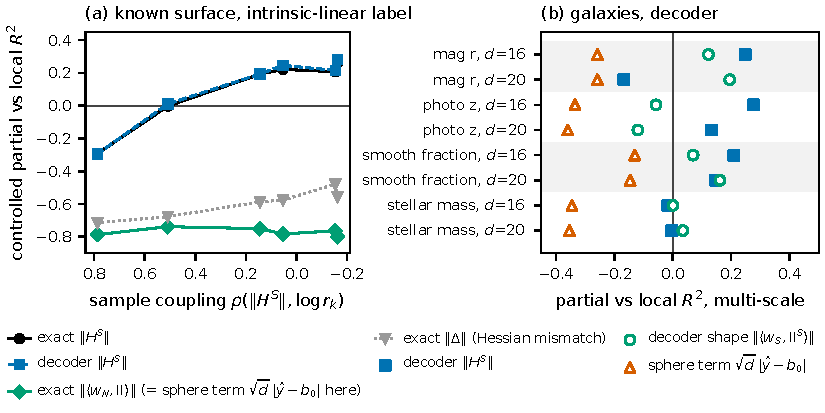
\includegraphics[width=0.85\textwidth]{figures/figF_mean_curvature.pdf}
\caption{(a) Known surface, linear label, exact geometry: three-control partial vs local $R^2$ as the density--curvature coupling is set by construction ($\gamma$ from $-1$ to $1$). (b) Galaxies, 512 anchors, $k=2{,}048$, multi-scale control: the decoder's $\norm{\Htan}$ (filled squares), shape term (open circles), sphere term (open triangles).}
\label{fig:meancurv}
\end{figure}
\end{document}
"` swaps Times for
% Computer Modern on machines without the Times metrics. CM is wider, so a 4-page fit here is
% conservative. Inactive on Overleaf and in the submitted build.
\ifdefined\LOCALFONTCHECK
  \renewcommand{\rmdefault}{cmr}\renewcommand{\sfdefault}{cmss}\renewcommand{\ttdefault}{cmtt}
\fi

\usepackage[utf8]{inputenc}
\usepackage[T1]{fontenc}
\usepackage{hyperref}
\usepackage{url}
\usepackage{booktabs}
\usepackage{amsmath,amssymb}
\usepackage{microtype}
\usepackage{xcolor}
\usepackage{graphicx}

\newcommand{\Htan}{H^{S}}
\newcommand{\norm}[1]{\lVert #1 \rVert}

\title{Linear Probes on Curved Latent Spaces}

\author{%
  Anonymous Author(s)\\
  Affiliation\\
  \texttt{email}
}

\begin{document}

\maketitle

\begin{abstract}
Linear probes are commonly used to evaluate learned representations and infer physical quantities for objects without direct measurements. However, their global predictive performance does not reveal where individual predictions are locally reliable or how the geometry of the learned representation contributes to their errors. Here we identify a geometric source of local readout error. Although a linear probe is affine in the ambient space, its restriction to a curved embedding manifold has a nonzero intrinsic Hessian given by $\langle w_N,\mathrm{II}\rangle$, the manifold's bending contracted with the probe's normal component. We turn this classical identity into a per-object measurement on galaxy embeddings from five encoders, using a decoder-based estimate of the second fundamental form validated on a synthetic surface of known curvature. Comparing this probe-facing curvature with the intrinsic Hessian of the physical target, we find that their mismatch predicts local readout accuracy for magnitude and photometric redshift, robustly under cross-fitting and across encoders. A counterfactual intervention on a local second-order surrogate further shows that reversing the probe-facing bending reduces local accuracy at nearly every anchor, whereas randomly oriented bending of matched strength does not exhibit the same asymmetry. The resulting tensor mismatch provides a geometric diagnostic of local linear-readout reliability and helps identify which physical quantities exhibit geometry-associated variation in prediction accuracy.
\end{abstract}

\section{Introduction}

Linear probes evaluate learned representations by measuring how accurately targets can be recovered from frozen embeddings~\citep{alain2017probes}. Their global performance, however, does not reveal where individual predictions are reliable or how representation geometry contributes to their errors. This matters in physical science, where probes infer quantities without direct measurements. For galaxy images, linear probes predict catalogue quantities such as magnitude, redshift and stellar mass~\citep{smith2024astropt}, but offer no local reliability diagnostic. We show that an ambient affine probe inherits curvature from the embedding manifold in its normal direction. The mismatch between this probe-facing curvature and the target's intrinsic Hessian captures a local source of prediction error.

We contribute (i) a decoder-based pointwise estimate of the second fundamental form, validated on a synthetic surface of known curvature; (ii) the application of the classical identity $\operatorname{Hess}_M(w\cdot x)=\langle w_N,\mathrm{II}\rangle$ to a fitted probe, with a residual expansion identifying its second-order approximation error; and (iii) evidence from 86{,}471 galaxies and five encoders that curvature mismatch predicts local readout accuracy for magnitude and redshift, supported by an intervention on a local second-order surrogate with a matched random-direction control.


\section{Pointwise curvature from a decoder}
\label{sec:instr}

\paragraph{Data.} 86{,}471 galaxies from the AstroPT galaxy set~\citep{smith2024astropt} with catalogue labels ($r$-band magnitude, photometric redshift, smooth fraction, stellar mass), embedded by a supervised ImageNet-21k ViT-B/16 (``ViT-B'' below) and by four further encoders (Section~\ref{sec:real}); embeddings from the Platonic Universe release~\citep{duraphe2025platonic}. We unit-normalize embeddings (data on $S^{D-1}$; $D=768$ for ViT-B).

\paragraph{Instrument.} Let $F:\mathbb{R}^d\to\mathbb{R}^{D}$ be the decoder of a plain auto-encoder (three hidden layers of width 250, SiLU), fit on 80\% of rows; we evaluate curvature on held-out rows. With $J = DF(z)$, metric $g = J^{\top}J$, normal projector $P_N = I - Jg^{-1}J^{\top}$ and second fundamental form $\mathrm{II} = P_N D^2F(z)$, all by automatic differentiation (cf.~\citep{lee2023curvature,acosta2023extrinsic}) at points where $DF$ has full column rank $d$. We differentiate the projected decoder $F/\norm{F}$, whose image lies on the unit sphere, so that $\mathrm{II}$ splits exactly into the sphere's universal radial part and an in-sphere shape part (Eq.~\eqref{eq:split}; Appendix~E).

\paragraph{Validation.} On a synthetic in-sphere surface at $D=768$ with closed-form $\mathrm{II}$ (Appendix~E), the decoder's estimate matches the true trace of $\mathrm{II}$ in direction (cosine 0.999), magnitude (ratio 1.00) and rank across points (0.94).

\section{What a linear readout sees on a curved manifold}
\label{sec:theory}


\paragraph{Notation.}
Let $M\subset\mathbb{R}^D$ be a $d$-dimensional
smooth embedded manifold, $d<D$, with anchor
$x_0\in M$. Let $J$ be an orthonormal tangent
frame at $x_0$ and $u$ normal coordinates in
this frame, so that locally
$x(u)=x_0+Ju+\tfrac12\mathrm{II}(u,u)
+O(\|u\|^3)$~\citep{lee2018riemannian}, where $\mathrm{II}$ is the
normal-valued second fundamental form. In
the numerical estimates, $J=DF$ is the
decoder Jacobian, with metric $g=J^\top J$,
and tangent-projected coordinates are used.
A probe weight decomposes as $w=w_T+w_N$
into tangent and normal components. On the
unit sphere, $\mathrm{II}=\mathrm{II}^S-g\,x$
separates the in-sphere shape from the
universal radial bending, and $w_S$ is
the component of $w_N$ orthogonal to $x$.
Let $y$ be a smooth target on $M$ and
$\hat y=w\cdot x+b_0$ a global affine probe.
Tensor norms and inner products use
$\langle A,B\rangle_g
=g^{ia}g^{jb}A_{ij}B_{ab}$.

Three facts follow. First, although the
probe is affine in the ambient space, its
restriction to $M$ is generally nonlinear
in intrinsic coordinates:
\begin{equation}
(d\hat y)_J=J^\top w,\qquad
\operatorname{Hess}_M\hat y
=\langle w_N,\mathrm{II}\rangle=:K.
\label{eq:hess}
\end{equation}
We call $K$ the probe-facing curvature.
Second, on the unit sphere it splits into
an in-sphere shape term and a radial term:
\begin{equation}
K=
\underbrace{\langle w_S,\mathrm{II}^S
\rangle}_{K_S}
+
\underbrace{[-(\hat y-b_0)g]}_{K_{\mathrm{sph}}}.
\label{eq:split}
\end{equation}
Thus, even an ambient affine readout
inherits intrinsic curvature from the
geometry of the representation.

Third, consider an isotropic Gaussian
patch $u\sim N(0,s^2I_d)$ in the
orthonormal tangent frame. For sufficiently
smooth embedding and target functions,
with controlled higher derivatives, let
$\bar c=\mathbb E_{\mathrm{patch}}[y-\hat y]$
be the patch-mean residual,
$\delta=(dy-d\hat y)_J$ the differential
mismatch, and
$\Delta=\operatorname{Hess}_M y-K$
the Hessian mismatch. Then
\begin{equation}
\begin{aligned}
\mathbb E_{\mathrm{patch}}
[(y-\hat y)^2]
={}&\bar c^{\,2}
+s^2\|\delta\|^2\\
&+\tfrac12s^4\|\Delta\|_g^2
+O(s^4\|\delta\|)+O(s^6).
\end{aligned}
\label{eq:resid}
\end{equation}
The Hessian mismatch therefore determines
the quadratic residual's contribution
to centered local error under this model.
Its contribution is smaller than at
$K=0$ iff
$2\langle\operatorname{Hess}_M y,K
\rangle_g>\|K\|_g^2$: the probe-facing
curvature must bend toward the target's
curvature, without overshooting it.
With the sphere term fixed, the
corresponding condition for the shape
term is
$2\langle R,K_S\rangle_g>\|K_S\|_g^2$,
where
$R=\operatorname{Hess}_M y-K_{\mathrm{sph}}$.
Section~\ref{sec:real} tests this
relationship. Since the quadratic
contribution scales as $s^4$, our
empirical analysis controls for
variation in local neighborhood scale.

\section{Probe-facing curvature: bending toward the label helps, bending away hurts}
\label{sec:real}

Statistic: five-fold out-of-fold ridge probe~\citep{alain2017probes} at the pre-registered $\alpha=100$ from embedding to label; local $R^2$ inside each of 512 anchors' 2{,}048-neighbourhoods; rank-partial Spearman against local $R^2$ with Freedman--Lane $p$-values~\citep{freedman1983permutation}, controlling for log patch radius, local label variance and count and, stronger, log radius at five scales.

\begin{figure}[t]
\centering
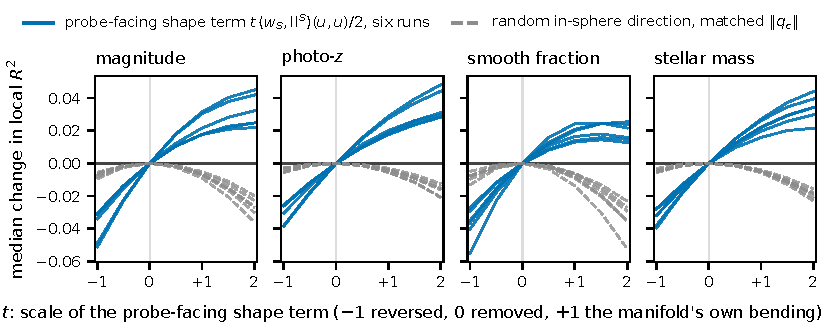
\includegraphics[width=\textwidth]{figures/fig1_intervention.pdf}
\caption{Bending toward the label helps, bending away hurts. At each of 512 anchors the readout's in-sphere shape quadratic $\tfrac t2\langle w_S,\mathrm{II}^S\rangle(u,u)$ is scaled by $t$ in a local second-order surrogate at a fixed manifold; lines are the median over anchors of the change in local $R^2$ relative to shape-flat ($t=0$). $t=1$ is the manifold's own bending seen from the readout's normal direction, $t=-1$ its reversal. Blue: the decoder's shape term, one line per run (five encoders at $d=16$, ViT-B also at $d=20$). Grey dashed: a random in-sphere normal direction with matched quadratic amplitude $\norm{q_c}$. Fractions of anchors helped and hurt, and sign tests on non-overlapping anchors, in Appendix~D.}
\label{fig:main}
\end{figure}

\paragraph{Galaxies.}
We estimate $\operatorname{Hess}_M y$ at each
anchor by fitting a least-squares quadratic
to the labels of its 2{,}048 neighbours in
tangent-projected coordinates
$u=g^{-1}J^\top(x-x_0)$. These decoder-based
Monge coordinates have vanishing Christoffel
symbols at the anchor, so the quadratic
coefficient estimates the covariant Hessian
in the small-neighbourhood limit. For
magnitude and redshift, the mismatch
$\|\Delta\|_g$ is negatively associated with
local $R^2$ ($-0.39$ to $-0.45$), while
alignment
$\cos_g(\operatorname{Hess}_M y,K)$
is positively associated with it
($+0.24$ to $+0.43$). These relationships
persist under cross-fitting (Appendix~B).
Smooth fraction exhibits weaker associations,
while stellar mass shows no significant
mismatch or alignment signal in this
experiment (Table~\ref{tab:real}; decoder
ablations, Appendix~A). Across five encoders, mismatch remains negatively associated with local accuracy for magnitude and redshift, while alignment is positive and significant for magnitude across all five and redshift across four (Appendix~C).

The shape term closely tracks the magnitude
of the total probe-facing curvature on
galaxies (rank correlation $0.96$--$0.99$),
but its association with local accuracy
varies across targets. This is consistent
with Eq.~\eqref{eq:resid}, where the shape
term's contribution to the quadratic
mismatch depends on both its magnitude and
its alignment with the remaining target
curvature. The sphere term is negatively
associated with local accuracy for all four
targets in the main ViT-B experiment,
although its association is sensitive to
probe regularization for some targets
(Appendix~E). Applying the same local
quadratic regression to the probe predictions
provides a decoder-independent estimate of
$K$, with median tensor cosine
$0.55$--$0.65$ relative to the
decoder-based estimate.

\paragraph{Relation to prior work.}
The identity in Eq.~\eqref{eq:hess} is
classical~\citep{milnor1963morse,chern1957total};
related work derives a curvature-dependent
normal weight for least-squares regression
on hypersurfaces~\citep{liu2023linear}
and documents the effects of curved
representations on linear
decoding~\citep{jurewicz2024irrational}.
Other approaches study manifold
capacity~\citep{chung2016linear,slatton2026linear},
representation flattening~\citep{psenka2024flattening},
curvature regularization~\citep{ma2023curvature},
latent geometry~\citep{kaufman2023latent},
local-regression bias~\citep{cheng2013local},
and geometric indicators of
generalization~\citep{chou2026diagnosing}.
Our contribution is to estimate the
pointwise probe-facing curvature tensor
on a learned manifold, compare it with
the target's intrinsic Hessian, and test
its contribution to local readout accuracy
through a controlled second-order intervention.

\paragraph{Bending toward helps, bending away hurts.}
To isolate the contribution of probe-facing
shape curvature, we intervene on the
in-sphere quadratic term of a local
second-order surrogate while keeping the
manifold, tangent readout, and sphere term
fixed. Each anchor's 2{,}048 neighbours
are scored by
$\hat y_t(u)=c+a^\top u+
\tfrac12K_{\mathrm{sph}}(u,u)+
\tfrac t2K_S(u,u)$,
where $a$ is the probe's tangent
differential, $K_S$ is estimated from the
decoder, and $c$ is refit for each $t$.
Here $t=1$ retains the estimated shape
quadratic of the original readout,
$t=-1$ reverses its sign, and $t=0$
removes it.

Under the isotropic Gaussian quadratic
model, $t=1$ improves upon $t=0$ iff
$2\langle R,K_S\rangle_g>\|K_S\|_g^2$.
On the actual neighbours, let $r_0$ be
the centred shape-flat residual and
$q_c$ the centred quadratic contribution
$\tfrac12K_S(u_i,u_i)$. After refitting
the intercept, the exact finite-sample
criterion is
$2\langle r_0,q_c\rangle>\|q_c\|^2$,
with optimum
$t^*=\langle r_0,q_c\rangle/\|q_c\|^2$
(Appendix~D).

Across five encoders and all four labels
(Figure~\ref{fig:main}), $t=1$ improves
local $R^2$ relative to the shape-flat
surrogate at 79--99\% of anchors, while
$t=-1$ reduces it at 97--100\%.
A random in-sphere normal direction with
matched centred quadratic amplitude shows
no comparable directional asymmetry and
is typically harmful under either sign
($t=1$ improves upon shape-flat at
22--36\% of anchors; Appendix~D).

Thus, the probe-selected shape quadratic
is locally error-reducing within the
second-order surrogate. Under the quadratic
Gaussian model, this is the signature of
bending toward the target's remaining
intrinsic curvature. This within-anchor
comparison differs from the cross-anchor
associations in Table~\ref{tab:real}
and can hold even where the latter show
no significant signal, as for stellar mass.
The optimum $t^*$ lies between 1.5 and
3.6 across runs, indicating that further
amplification of the shape term reduces
local surrogate error. 

\section{Discussion}

Our results identify a geometric source of local linear-probe error: the mismatch $\Delta=\operatorname{Hess}_M y-\langle w_N,\mathrm{II}\rangle$ between the target's intrinsic Hessian and the curvature induced by the probe. We estimate this mismatch using a decoder-based second fundamental form, validated on a synthetic surface and showing moderate agreement with a decoder-independent estimate on galaxy embeddings. Across five encoders, mismatch tracks local accuracy for magnitude and redshift, with weaker evidence for smooth fraction. A counterfactual intervention on the local second-order surrogate shows that the probe-selected shape term reduces error at most anchors, while reversing it generally increases error. Thus, manifold curvature can help rather than hinder linear decoding when it bends toward the target's curvature.

The mismatch can be estimated from labelled neighbours without knowing an object's target value, providing a local diagnostic of predictions that may warrant further scrutiny. It is not yet a calibrated per-object uncertainty estimate. For stellar mass, mismatch does not consistently track local accuracy despite the beneficial shape contribution, showing that a locally useful geometric effect need not explain variation in overall readout accuracy.

\emph{Limitations.}
We study one galaxy sample, four targets and five encoders. The label Hessian is estimated from finite neighbourhoods; its norm is reliably ranked (split-half $\rho=0.91$--$0.94$), but its direction is only moderately recovered (tensor cosine $0.19$--$0.35$). The synthetic surface does not independently corroborate the alignment association because its target has insufficient intrinsic curvature. The intervention modifies a local surrogate, not the encoder or manifold. Mismatch and alignment are the primary hypotheses; other analyses are exploratory. Overlapping neighbourhoods introduce anchor dependence that may affect permutation-test validity.

\bibliographystyle{unsrtnat}
{\small
\bibliography{references}
}

\appendix
% BEGIN APPENDIX AUTOGEN
\section*{Appendix A: decoder ablations}
Table~\ref{tab:ablate} repeats the four quantities of Tables~\ref{tab:real} and~\ref{tab:meancurv} at $d=16$ under the multi-scale density control for two further decoder initialisation seeds and for a decoder of width $400^3$ instead of $250^3$ (all fits reach variance explained 0.952). Every significant sign of the main table is retained.
\begin{table}[h]
\centering\footnotesize\setlength{\tabcolsep}{4pt}
\begin{tabular}{llcccc}
\toprule
label & quantity & seed 0 & seed 1 & seed 2 & $400^3$ \\
\midrule
mag\_r & shape & $+0.12$ & $+0.05^{*}$ & $+0.12$ & $+0.05^{*}$ \\
 & sphere & $-0.26$ & $-0.26$ & $-0.27$ & $-0.26$ \\
 & mismatch & $-0.39$ & $-0.35$ & $-0.34$ & $-0.34$ \\
 & alignment & $+0.35$ & $+0.31$ & $+0.37$ & $+0.41$ \\
\addlinespace[2pt]
photo\_z & shape & $-0.06^{*}$ & $-0.09^{*}$ & $-0.09$ & $-0.06^{*}$ \\
 & sphere & $-0.33$ & $-0.35$ & $-0.34$ & $-0.35$ \\
 & mismatch & $-0.45$ & $-0.43$ & $-0.42$ & $-0.41$ \\
 & alignment & $+0.26$ & $+0.24$ & $+0.25$ & $+0.25$ \\
\addlinespace[2pt]
smooth\_fraction & shape & $+0.07^{*}$ & $+0.20$ & $+0.15$ & $+0.10$ \\
 & sphere & $-0.13$ & $-0.15$ & $-0.14$ & $-0.11$ \\
 & mismatch & $-0.09^{*}$ & $-0.05^{*}$ & $-0.08^{*}$ & $-0.07^{*}$ \\
 & alignment & $+0.19$ & $+0.14$ & $+0.09$ & $+0.10$ \\
\addlinespace[2pt]
stellar\_mass & shape & $+0.00^{*}$ & $-0.06^{*}$ & $+0.05^{*}$ & $+0.09$ \\
 & sphere & $-0.35$ & $-0.35$ & $-0.35$ & $-0.35$ \\
 & mismatch & $-0.04^{*}$ & $+0.03^{*}$ & $+0.02^{*}$ & $+0.03^{*}$ \\
 & alignment & $+0.01^{*}$ & $-0.02^{*}$ & $+0.03^{*}$ & $-0.02^{*}$ \\
\addlinespace[2pt]
\bottomrule
\end{tabular}
\caption{Decoder ablations, $d=16$, 512 anchors, multi-scale density control. $^{*}$ not significant at 0.05.}
\label{tab:ablate}
\end{table}
\section*{Appendix B: sensitivity of the mismatch and sphere columns}
Cross-fitting: each 2{,}048-patch is split at random into halves; $\operatorname{Hess}_M y$ is fitted on one half and local $R^2$ scored on the other (both directions shown), so the Hessian estimate and the outcome share no rows. The split-half cosine between the two Hessian estimates is the reliability of the estimate. Weak ridge: the probe refit at $\alpha=1$ instead of 100 (global out-of-sample $R^2$ rises by 0.10 to 0.15), which substantially reduces the shrinkage of extreme predictions; the sphere term is recomputed from that probe.
\begin{table}[h]
\centering\footnotesize\setlength{\tabcolsep}{3.5pt}
\begin{tabular}{llcccccc}
\toprule
 & & \multicolumn{2}{c}{mismatch, cross-fit} & \multicolumn{2}{c}{alignment, cross-fit} & Hess.\ split cos & sphere, $\alpha=1$ \\
label & $d$ & fit A/score B & fit B/score A & fit A/score B & fit B/score A & p50 & (main: $\alpha=100$) \\
\midrule
mag\_r & 16 & $-0.38$ & $-0.34$ & $+0.33$ & $+0.31$ & +0.35 & $-0.21$ ($-0.26$) \\
mag\_r & 20 & $-0.43$ & $-0.40$ & $+0.39$ & $+0.37$ & +0.24 & $-0.22$ ($-0.26$) \\
photo\_z & 16 & $-0.42$ & $-0.36$ & $+0.23$ & $+0.20$ & +0.32 & $+0.05^{*}$ ($-0.33$) \\
photo\_z & 20 & $-0.42$ & $-0.42$ & $+0.22$ & $+0.22$ & +0.20 & $+0.03^{*}$ ($-0.36$) \\
smooth\_fraction & 16 & $-0.10$ & $-0.17$ & $+0.17$ & $+0.19$ & +0.33 & $-0.12$ ($-0.13$) \\
smooth\_fraction & 20 & $-0.15$ & $-0.21$ & $+0.05^{*}$ & $+0.03^{*}$ & +0.23 & $-0.13$ ($-0.15$) \\
stellar\_mass & 16 & $+0.01^{*}$ & $-0.04^{*}$ & $-0.03^{*}$ & $+0.06^{*}$ & +0.31 & $-0.02^{*}$ ($-0.35$) \\
stellar\_mass & 20 & $-0.06^{*}$ & $-0.07^{*}$ & $+0.01^{*}$ & $-0.00^{*}$ & +0.19 & $-0.02^{*}$ ($-0.35$) \\
\bottomrule
\end{tabular}
\caption{Cross-fitted mismatch and alignment partials (multi-scale control), split-half reliability of the label Hessian, and the sphere-term partial under a weak-ridge probe.}
\label{tab:sens}
\end{table}

\section*{Appendix C: Main and cross-encoder results}

\paragraph{Main results.}
Table~\ref{tab:real} reports the associations
between geometric mismatch, alignment and local
readout accuracy for ViT-B at $d=16$ and $d=20$.
Results use 512 anchors, $k=2{,}048$ neighbours
and the multi-scale density control.

\begin{table}[h]
\centering
\footnotesize
\setlength{\tabcolsep}{3.4pt}
\begin{tabular}{lcccc}
\toprule
 & \multicolumn{2}{c}{mismatch $\norm{\Delta}_g$}
 & \multicolumn{2}{c}{alignment $\cos_g(\operatorname{Hess}_M y, K)$} \\
label & $d{=}16$ & $d{=}20$ & $d{=}16$ & $d{=}20$ \\
\midrule
mag\_r & $-0.39$ & $-0.40$ & $+0.35$ & $+0.43$ \\
photo\_z & $-0.45$ & $-0.44$ & $+0.26$ & $+0.24$ \\
smooth\_fraction & $-0.09^{*}$ & $-0.17$ & $+0.19$ & $+0.07^{*}$ \\
stellar\_mass & $-0.04^{*}$ & $-0.09^{*}$ & $+0.01^{*}$ & $+0.02^{*}$ \\
\bottomrule
\end{tabular}
\caption{ViT-B: rank-partial Spearman correlations
with local $R^2$ under the multi-scale density
control. $^{*}$ Not significant at 0.05.
Shape, sphere and mean-curvature results
are reported in Appendix~E.}
\label{tab:real}
\end{table}

\paragraph{Across encoders.}
We repeat the geometric diagnostic at $d=16$
on the same 86{,}471 galaxies using four further
encoders from the Platonic Universe release:
DINOv3 ViT-B/16, CLIP ViT-B, ConvNeXt-B and
ViT-L (widths 768, 512, 1{,}024 and 1{,}024;
all unit-normalized).
A decoder of the same architecture and training
protocol is fitted per encoder (seed 0;
variance explained 0.966, 0.985, 0.965 and
0.968, respectively). All analyses use
512 anchors, $k=2{,}048$ and the multi-scale
density control.

For magnitude and redshift, mismatch is
negatively associated with local $R^2$
across all five encoders ($-0.32$ to $-0.61$;
cross-fitted $-0.28$ to $-0.62$).
Alignment is positive and significant for
magnitude across all five ($+0.13$ to $+0.53$)
and for redshift across four.
Shape-term associations vary by encoder and
target, while smooth fraction shows less
consistent mismatch and alignment signals.
For stellar mass, alignment is nonsignificant
across encoders and mismatch significant in
only one main comparison. Thus, the
cross-anchor mismatch association varies by
target, even where the shape term improves
the local surrogate.

Table~\ref{tab:xenc} reports the full
cross-encoder results, including global
out-of-sample probe $R^2$ in the first row
for each label. Table~\ref{tab:xencx}
reports cross-fitted mismatch and alignment
associations and split-half reliability of
the estimated label Hessian.

\begin{table}[h]
\centering
\footnotesize
\setlength{\tabcolsep}{4pt}
\begin{tabular}{llccccc}
\toprule
label & quantity & ViT-B & DINOv3 & CLIP-B & ConvNeXt-B & ViT-L \\
\midrule
mag\_r & global $R^2$ & 0.52 & 0.57 & 0.50 & 0.52 & 0.52 \\
 & shape & $+0.12$ & $-0.11$ & $+0.16$ & $+0.16$ & $-0.21$ \\
 & sphere & $-0.26$ & $-0.23$ & $-0.40$ & $-0.24$ & $-0.08^{*}$ \\
 & mismatch & $-0.39$ & $-0.57$ & $-0.34$ & $-0.32$ & $-0.44$ \\
 & alignment & $+0.35$ & $+0.53$ & $+0.32$ & $+0.21$ & $+0.13$ \\
\addlinespace[2pt]
photo\_z & global $R^2$ & 0.51 & 0.56 & 0.49 & 0.49 & 0.51 \\
 & shape & $-0.06^{*}$ & $-0.05^{*}$ & $-0.17$ & $+0.29$ & $-0.16$ \\
 & sphere & $-0.33$ & $-0.21$ & $-0.29$ & $-0.46$ & $-0.44$ \\
 & mismatch & $-0.45$ & $-0.61$ & $-0.45$ & $-0.48$ & $-0.46$ \\
 & alignment & $+0.26$ & $+0.33$ & $+0.06^{*}$ & $+0.22$ & $+0.14$ \\
\addlinespace[2pt]
smooth\_fraction & global $R^2$ & 0.53 & 0.59 & 0.49 & 0.56 & 0.55 \\
 & shape & $+0.07^{*}$ & $-0.08^{*}$ & $+0.20$ & $+0.24$ & $+0.06^{*}$ \\
 & sphere & $-0.13$ & $-0.06^{*}$ & $+0.05^{*}$ & $-0.15$ & $-0.11$ \\
 & mismatch & $-0.09^{*}$ & $-0.33$ & $-0.25$ & $-0.20$ & $-0.01^{*}$ \\
 & alignment & $+0.19$ & $-0.02^{*}$ & $+0.24$ & $+0.04^{*}$ & $+0.14$ \\
\addlinespace[2pt]
stellar\_mass & global $R^2$ & 0.48 & 0.54 & 0.50 & 0.49 & 0.49 \\
 & shape & $+0.00^{*}$ & $-0.15$ & $-0.10$ & $-0.11$ & $-0.13$ \\
 & sphere & $-0.35$ & $-0.26$ & $-0.38$ & $-0.40$ & $-0.38$ \\
 & mismatch & $-0.04^{*}$ & $+0.03^{*}$ & $-0.12$ & $-0.06^{*}$ & $-0.02^{*}$ \\
 & alignment & $+0.01^{*}$ & $-0.05^{*}$ & $-0.01^{*}$ & $+0.07^{*}$ & $-0.03^{*}$ \\
\addlinespace[2pt]
\bottomrule
\end{tabular}
\caption{Cross-encoder results at $d=16$:
global probe $R^2$ and rank-partial Spearman
correlations with local $R^2$ under the
multi-scale density control.
$^{*}$ Not significant at 0.05.}
\label{tab:xenc}
\end{table}

\begin{table}[h]
\centering
\footnotesize
\setlength{\tabcolsep}{3.5pt}
\begin{tabular}{llccccc}
\toprule
 & & \multicolumn{2}{c}{mismatch, cross-fit}
 & \multicolumn{2}{c}{alignment, cross-fit}
 & Hess.\ split cos \\
encoder & label & fit A/score B & fit B/score A
& fit A/score B & fit B/score A & p50 \\
\midrule
\addlinespace[2pt]
DINOv3 & mag\_r & $-0.60$ & $-0.62$ & $+0.50$ & $+0.50$ & +0.35 \\
 & photo\_z & $-0.56$ & $-0.59$ & $+0.28$ & $+0.27$ & +0.24 \\
 & smooth\_fraction & $-0.32$ & $-0.29$ & $-0.03^{*}$ & $-0.02^{*}$ & +0.31 \\
 & stellar\_mass & $+0.03^{*}$ & $+0.02^{*}$ & $-0.03^{*}$ & $-0.07^{*}$ & +0.22 \\
\addlinespace[2pt]
CLIP-B & mag\_r & $-0.28$ & $-0.35$ & $+0.28$ & $+0.29$ & +0.31 \\
 & photo\_z & $-0.41$ & $-0.40$ & $+0.08^{*}$ & $+0.06^{*}$ & +0.25 \\
 & smooth\_fraction & $-0.22$ & $-0.24$ & $+0.15$ & $+0.20$ & +0.28 \\
 & stellar\_mass & $-0.14$ & $-0.13$ & $-0.04^{*}$ & $+0.01^{*}$ & +0.19 \\
\addlinespace[2pt]
ConvNeXt-B & mag\_r & $-0.36$ & $-0.34$ & $+0.19$ & $+0.21$ & +0.29 \\
 & photo\_z & $-0.46$ & $-0.45$ & $+0.18$ & $+0.19$ & +0.30 \\
 & smooth\_fraction & $-0.15$ & $-0.19$ & $-0.02^{*}$ & $+0.03^{*}$ & +0.32 \\
 & stellar\_mass & $-0.05^{*}$ & $-0.01^{*}$ & $+0.14$ & $-0.03^{*}$ & +0.29 \\
\addlinespace[2pt]
ViT-L & mag\_r & $-0.46$ & $-0.49$ & $+0.09^{*}$ & $+0.15$ & +0.30 \\
 & photo\_z & $-0.44$ & $-0.42$ & $+0.09^{*}$ & $+0.13$ & +0.24 \\
 & smooth\_fraction & $-0.03^{*}$ & $-0.04^{*}$ & $+0.11$ & $+0.07^{*}$ & +0.30 \\
 & stellar\_mass & $-0.06^{*}$ & $+0.01^{*}$ & $-0.04^{*}$ & $-0.03^{*}$ & +0.21 \\
\addlinespace[2pt]
\bottomrule
\end{tabular}
\caption{Cross-fitted mismatch and alignment
partials under the multi-scale density
control, with median split-half tensor
cosine for the estimated label Hessian.
$^{*}$ Not significant at 0.05.}
\label{tab:xencx}
\end{table}
\section*{Appendix D: intervening on the readout's normal component}
The partials of Table~\ref{tab:real} compare anchors with one another and cannot say whether reversing the probe-facing shape term hurts relative to removing it, since no anchor is flat. Here we score a counterfactual local second-order surrogate of the readout at a fixed manifold. At each anchor the fitted ridge weight is split into tangent, radial and in-sphere normal parts $w = w_T + w_{\mathrm{rad}} + w_S$; we score the anchor's 2{,}048 neighbours by the data-side tangent-plus-sphere readout $(w_T + w_{\mathrm{rad}})\cdot x$ plus $t\,q$ with the local intercept refit, where $q = \tfrac12\langle w_S,\mathrm{II}^S\rangle(u,u)$ is the decoder's in-sphere second-order term in the anchor's chart coordinates: $t=1$ is the manifold's bending as seen in the readout's normal direction, $t=-1$ its sign reversal, $t=0$ shape-flat (the sphere term $-(w\!\cdot\!\hat x)g$ is kept in the base). Because the intercept is refit for every $t$, the local sum of squares is exactly $\mathrm{SSE}(t) = \norm{r_0 - t\,q_c}^2$ with $r_0$ the centred residual of the shape-flat predictor and $q_c = q - \bar q\mathbf 1$ the centred quadratic on the anchor's neighbours; hence $t^{*} = \langle r_0,q_c\rangle/\norm{q_c}^2$ and $t=1$ beats shape-flat iff $2\langle r_0,q_c\rangle > \norm{q_c}^2$. This is the finite-sample counterpart of the tensor-level condition $2\langle R,K_S\rangle_g > \norm{K_S}_g^2$ of Section~\ref{sec:theory}, not the same quantity: the tensor version needs the estimated label Hessian, the empirical one does not. Columns: fraction of anchors where $t=1$ beats shape-flat (help) and where $t=-1$ is worse than shape-flat (hurt), the median change in local $R^2$ at $t=\pm1$, the median $t^{*}$; then the same for a random in-sphere normal direction $v$ whose quadratic is rescaled to the same centred amplitude on the actual neighbours, $\norm{q_{v,c}} = \norm{q_c}$ (matching $\norm{v}$ to $\norm{w_S}$ instead leaves the contracted tensor at a fraction of the fitted one, since $\mathrm{II}^S$ spans at most $d(d+1)/2$ of the $\sim 750$ normal directions; matching $\norm{\langle v,\mathrm{II}^S\rangle}_g$ gives the same picture; Supplement 12). The anchors' neighbourhoods overlap (each point lies in about twelve of them), so the fractions are not counts of independent trials; a maximal set of anchors whose pairwise overlap is at most 5\% of $k$ has 19--21 members per run, on which $t=1$ beats shape-flat at 81--100\% (one-sided sign test $p \le 4\times 10^{-3}$ in every cell) and $t=-1$ is worse at 95--100\% ($p \le 3\times 10^{-5}$).
\begin{table}[h]
\centering\footnotesize\setlength{\tabcolsep}{3pt}
\begin{tabular}{llccccc|cccc}
\toprule
 & & \multicolumn{5}{c|}{decoder in-sphere shape term} & \multicolumn{4}{c}{random orientation, matched $\norm{q_c}$} \\
run & label & help & hurt & $\Delta R^2(+1)$ & $\Delta R^2(-1)$ & $t^{*}$ & help & hurt & $\Delta R^2(+1)$ & $\Delta R^2(-1)$ \\
\midrule
ViT-B, $d=16$ & mag\_r & 0.97 & 1.00 & $+0.030$ & $-0.051$ & 2.3 & 0.26 & 0.80 & $-0.009$ & $-0.009$ \\
 & photo\_z & 0.99 & 0.99 & $+0.028$ & $-0.038$ & 3.0 & 0.33 & 0.68 & $-0.005$ & $-0.006$ \\
 & smooth\_fraction & 0.90 & 1.00 & $+0.021$ & $-0.040$ & 1.7 & 0.24 & 0.78 & $-0.008$ & $-0.010$ \\
 & stellar\_mass & 0.96 & 0.99 & $+0.026$ & $-0.040$ & 2.6 & 0.29 & 0.70 & $-0.006$ & $-0.006$ \\
\addlinespace[2pt]
ViT-B, $d=20$ & mag\_r & 0.99 & 1.00 & $+0.031$ & $-0.049$ & 2.6 & 0.24 & 0.78 & $-0.007$ & $-0.008$ \\
 & photo\_z & 0.99 & 1.00 & $+0.029$ & $-0.038$ & 3.6 & 0.36 & 0.71 & $-0.004$ & $-0.005$ \\
 & smooth\_fraction & 0.90 & 1.00 & $+0.020$ & $-0.035$ & 1.9 & 0.22 & 0.77 & $-0.007$ & $-0.008$ \\
 & stellar\_mass & 0.97 & 1.00 & $+0.027$ & $-0.038$ & 3.1 & 0.32 & 0.72 & $-0.005$ & $-0.005$ \\
\addlinespace[2pt]
DINOv3, $d=16$ & mag\_r & 0.92 & 0.99 & $+0.018$ & $-0.031$ & 2.0 & 0.29 & 0.71 & $-0.007$ & $-0.006$ \\
 & photo\_z & 0.96 & 0.99 & $+0.020$ & $-0.030$ & 2.6 & 0.29 & 0.71 & $-0.006$ & $-0.004$ \\
 & smooth\_fraction & 0.93 & 1.00 & $+0.024$ & $-0.055$ & 1.5 & 0.22 & 0.78 & $-0.014$ & $-0.013$ \\
 & stellar\_mass & 0.95 & 1.00 & $+0.016$ & $-0.028$ & 2.1 & 0.26 & 0.74 & $-0.005$ & $-0.005$ \\
\addlinespace[2pt]
CLIP-B, $d=16$ & mag\_r & 0.95 & 0.99 & $+0.018$ & $-0.031$ & 2.2 & 0.30 & 0.68 & $-0.006$ & $-0.005$ \\
 & photo\_z & 0.99 & 1.00 & $+0.019$ & $-0.026$ & 3.4 & 0.36 & 0.64 & $-0.003$ & $-0.003$ \\
 & smooth\_fraction & 0.92 & 0.99 & $+0.014$ & $-0.027$ & 1.7 & 0.25 & 0.69 & $-0.006$ & $-0.005$ \\
 & stellar\_mass & 0.97 & 1.00 & $+0.020$ & $-0.028$ & 2.8 & 0.35 & 0.68 & $-0.004$ & $-0.005$ \\
\addlinespace[2pt]
ConvNeXt-B, $d=16$ & mag\_r & 0.92 & 1.00 & $+0.018$ & $-0.031$ & 2.0 & 0.26 & 0.73 & $-0.007$ & $-0.007$ \\
 & photo\_z & 0.99 & 1.00 & $+0.018$ & $-0.026$ & 2.9 & 0.28 & 0.64 & $-0.004$ & $-0.003$ \\
 & smooth\_fraction & 0.88 & 0.98 & $+0.016$ & $-0.036$ & 1.6 & 0.23 & 0.75 & $-0.009$ & $-0.008$ \\
 & stellar\_mass & 0.99 & 1.00 & $+0.022$ & $-0.032$ & 3.1 & 0.29 & 0.65 & $-0.005$ & $-0.003$ \\
\addlinespace[2pt]
ViT-L, $d=16$ & mag\_r & 0.96 & 0.99 & $+0.022$ & $-0.034$ & 2.6 & 0.32 & 0.74 & $-0.005$ & $-0.006$ \\
 & photo\_z & 0.97 & 0.99 & $+0.018$ & $-0.025$ & 3.2 & 0.34 & 0.67 & $-0.004$ & $-0.003$ \\
 & smooth\_fraction & 0.79 & 0.97 & $+0.013$ & $-0.029$ & 1.6 & 0.25 & 0.77 & $-0.006$ & $-0.008$ \\
 & stellar\_mass & 0.98 & 1.00 & $+0.022$ & $-0.032$ & 2.9 & 0.30 & 0.67 & $-0.004$ & $-0.004$ \\
\addlinespace[2pt]
\bottomrule
\end{tabular}
\caption{Counterfactual scaling of the in-sphere shape term in a local second-order surrogate of the readout, 512 anchors per run. The manifold's bending as seen in the readout's normal direction helps at a large majority of anchors, its sign reversal hurts at nearly every anchor, a random orientation of the same centred quadratic amplitude shows no such asymmetry and is typically harmful under either sign; $t^{*}>1$ throughout, consistent with the globally ridge-regularized probe under-using a locally beneficial term.}
\label{tab:cf}
\end{table}
% END APPENDIX AUTOGEN

% Appendix E is hand-written (not generated); numbers are the same record-verified values that stood in the main text until 2026-09-18.
\section*{Appendix E: the shape and sphere terms, and mean curvature}
\label{app:meancurv}
The mean-curvature vector of the decoder surface is $H = \operatorname{tr}_g \mathrm{II}$ (unnormalized trace; some authors divide by $d$). Alongside Eq.~\eqref{eq:hess}, $\Delta_M (w\!\cdot\! x) = \langle w, H\rangle$: the Laplacian of a linear readout sees only the trace of $\mathrm{II}$, its Hessian the whole tensor, so $\norm{H}$ need not track $\langle w_N,\mathrm{II}\rangle$. On the unit sphere the Euclidean mean-curvature vector of every $d$-submanifold has the universal radial component $-d\,\hat x$, which says nothing about shape; differentiating the projected decoder $F/\norm{F}$ splits $H = -d\,\hat x + \Htan$ exactly (radial part $-d$ to $10^{-14}$), and $\Htan$ is the non-radial mean-curvature component used below.

\emph{Validation surface.} At $D=768$ the in-sphere surface $G(z) = Q\,\mathrm{normalize}([\phi(z);\,0.8\,h(z);\,0\ldots])$ ($\phi$ inverse stereographic $\mathbb{R}^{16}\to S^{16}$, $h$ four Gaussian bumps, $Q$ a rotation) has closed-form curvature; the decoder's $\Htan$ gives rank 0.94 against the true $\norm{\Htan}$, direction cosine 0.999, magnitude ratio 1.00. Resampling this surface with weight $\norm{\Htan}^\gamma$ (Figure~\ref{fig:meancurv}a) moves the density-controlled $\norm{\Htan}$ partial against local $R^2$ from $-0.29$ to $+0.26$, while $\norm{\langle w_N,\mathrm{II}\rangle}_g$ holds at $-0.74$ to $-0.80$, dominated by the sphere term of Eq.~\eqref{eq:split}; the mismatch partial reproduces there, the alignment partial has no stable sign.

\emph{Galaxies: shape and sphere terms.} Table~\ref{tab:meancurv} gives the density-controlled partials of the two terms of Eq.~\eqref{eq:split} against local $R^2$ (Figure~\ref{fig:meancurv}b). The shape term dominates the probe-facing Hessian on galaxies (rank $0.96$--$0.99$ with $\norm{K}_g$) and is label-signed: positive for magnitude and smooth fraction, null to weakly negative for redshift, null for stellar mass. The sphere term is negative on every label and both $d$ ($-0.13$ to $-0.36$) under the $\alpha=100$ probe; with a weak-ridge probe ($\alpha=1$, Appendix~B) it stays negative for magnitude and smooth fraction ($-0.21$, $-0.12$) and vanishes for redshift and stellar mass, so part of it is ridge shrinkage of extreme predictions rather than geometry.

\emph{Galaxies: mean curvature.} The $\norm{\Htan}$ partial changes sign with the latent dimension for magnitude and is null for stellar mass. Across the five encoders of Appendix~C the quadratic-chart mean-bending trace has density-controlled associations with the magnitude probe's local $R^2$ of both signs ($-0.24$ to $+0.27$), as Eq.~\eqref{eq:hess} allows. Mean curvature, the scalar usually reported, keeps only the trace of $\mathrm{II}$ and fails accordingly: its association with readout accuracy changes sign with the sampling on the known surface and with the latent dimension and the encoder on galaxies.
\begin{table}[h]
\centering\footnotesize\setlength{\tabcolsep}{4pt}
\begin{tabular}{lcccccc}
\toprule
 & \multicolumn{2}{c}{shape $\norm{\langle w_S,\mathrm{II}^S\rangle}$} & \multicolumn{2}{c}{sphere $\sqrt d\,|\hat y-b_0|$} & \multicolumn{2}{c}{$\norm{\Htan}$} \\
label & $d{=}16$ & $d{=}20$ & 16 & 20 & 16 & 20 \\
\midrule
mag\_r & $+0.12$ & $+0.19$ & $-0.26$ & $-0.26$ & $+0.25$ & $-0.17$ \\
photo\_z & $-0.06^{*}$ & $-0.12$ & $-0.33$ & $-0.36$ & $+0.28$ & $+0.13$ \\
smooth\_fraction & $+0.07^{*}$ & $+0.16$ & $-0.13$ & $-0.15$ & $+0.21$ & $+0.15$ \\
stellar\_mass & $+0.00^{*}$ & $+0.03^{*}$ & $-0.35$ & $-0.35$ & $-0.02^{*}$ & $-0.00^{*}$ \\
\bottomrule
\end{tabular}
\caption{Galaxies, 512 anchors, $k=2{,}048$, multi-scale density control: rank-partial Spearman against local $R^2$ of the shape term, the sphere term and the scalar $\norm{\Htan}$. $^{*}$ not significant at 0.05.}
\label{tab:meancurv}
\end{table}
\begin{figure}[h]
\centering
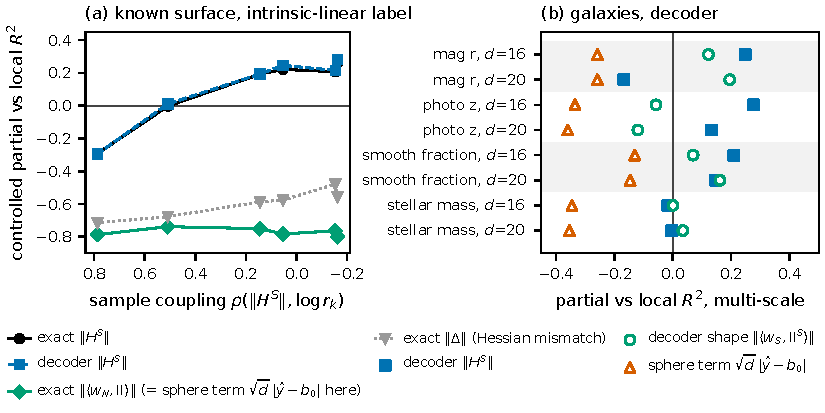
\includegraphics[width=0.85\textwidth]{figures/figF_mean_curvature.pdf}
\caption{(a) Known surface, linear label, exact geometry: three-control partial vs local $R^2$ as the density--curvature coupling is set by construction ($\gamma$ from $-1$ to $1$). (b) Galaxies, 512 anchors, $k=2{,}048$, multi-scale control: the decoder's $\norm{\Htan}$ (filled squares), shape term (open circles), sphere term (open triangles).}
\label{fig:meancurv}
\end{figure}
\end{document}
"` swaps Times for
% Computer Modern on machines without the Times metrics. CM is wider, so a 4-page fit here is
% conservative. Inactive on Overleaf and in the submitted build.
\ifdefined\LOCALFONTCHECK
  \renewcommand{\rmdefault}{cmr}\renewcommand{\sfdefault}{cmss}\renewcommand{\ttdefault}{cmtt}
\fi

\usepackage[utf8]{inputenc}
\usepackage[T1]{fontenc}
\usepackage{hyperref}
\usepackage{url}
\usepackage{booktabs}
\usepackage{amsmath,amssymb}
\usepackage{microtype}
\usepackage{xcolor}
\usepackage{graphicx}

\newcommand{\Htan}{H^{S}}
\newcommand{\norm}[1]{\lVert #1 \rVert}

\title{Linear Probes on Curved Latent Spaces}

\author{%
  Anonymous Author(s)\\
  Affiliation\\
  \texttt{email}
}

\begin{document}

\maketitle

\begin{abstract}
Linear probes are commonly used to evaluate learned representations and infer physical quantities for objects without direct measurements. However, their global predictive performance does not reveal where individual predictions are locally reliable or how the geometry of the learned representation contributes to their errors. Here we identify a geometric source of local readout error. Although a linear probe is affine in the ambient space, its restriction to a curved embedding manifold has a nonzero intrinsic Hessian given by $\langle w_N,\mathrm{II}\rangle$, the manifold's bending contracted with the probe's normal component. We turn this classical identity into a per-object measurement on galaxy embeddings from five encoders, using a decoder-based estimate of the second fundamental form validated on a synthetic surface of known curvature. Comparing this probe-facing curvature with the intrinsic Hessian of the physical target, we find that their mismatch predicts local readout accuracy for magnitude and photometric redshift, robustly under cross-fitting and across encoders. A counterfactual intervention on a local second-order surrogate further shows that reversing the probe-facing bending reduces local accuracy at nearly every anchor, whereas randomly oriented bending of matched strength does not exhibit the same asymmetry. The resulting tensor mismatch provides a geometric diagnostic of local linear-readout reliability and helps identify which physical quantities exhibit geometry-associated variation in prediction accuracy.
\end{abstract}

\section{Introduction}

Linear probes evaluate learned representations by measuring how accurately targets can be recovered from frozen embeddings~\citep{alain2017probes}. Their global performance, however, does not reveal where individual predictions are reliable or how representation geometry contributes to their errors. This matters in physical science, where probes infer quantities without direct measurements. For galaxy images, linear probes predict catalogue quantities such as magnitude, redshift and stellar mass~\citep{smith2024astropt}, but offer no local reliability diagnostic. We show that an ambient affine probe inherits curvature from the embedding manifold in its normal direction. The mismatch between this probe-facing curvature and the target's intrinsic Hessian captures a local source of prediction error.

We contribute (i) a decoder-based pointwise estimate of the second fundamental form, validated on a synthetic surface of known curvature; (ii) the application of the classical identity $\operatorname{Hess}_M(w\cdot x)=\langle w_N,\mathrm{II}\rangle$ to a fitted probe, with a residual expansion identifying its second-order approximation error; and (iii) evidence from 86{,}471 galaxies and five encoders that curvature mismatch predicts local readout accuracy for magnitude and redshift, supported by an intervention on a local second-order surrogate with a matched random-direction control.


\section{Pointwise curvature from a decoder}
\label{sec:instr}

\paragraph{Data.} 86{,}471 galaxies from the AstroPT galaxy set~\citep{smith2024astropt} with catalogue labels ($r$-band magnitude, photometric redshift, smooth fraction, stellar mass), embedded by a supervised ImageNet-21k ViT-B/16 (``ViT-B'' below) and by four further encoders (Section~\ref{sec:real}); embeddings from the Platonic Universe release~\citep{duraphe2025platonic}. We unit-normalize embeddings (data on $S^{D-1}$; $D=768$ for ViT-B).

\paragraph{Instrument.} Let $F:\mathbb{R}^d\to\mathbb{R}^{D}$ be the decoder of a plain auto-encoder (three hidden layers of width 250, SiLU), fit on 80\% of rows; we evaluate curvature on held-out rows. With $J = DF(z)$, metric $g = J^{\top}J$, normal projector $P_N = I - Jg^{-1}J^{\top}$ and second fundamental form $\mathrm{II} = P_N D^2F(z)$, all by automatic differentiation (cf.~\citep{lee2023curvature,acosta2023extrinsic}) at points where $DF$ has full column rank $d$. We differentiate the projected decoder $F/\norm{F}$, whose image lies on the unit sphere, so that $\mathrm{II}$ splits exactly into the sphere's universal radial part and an in-sphere shape part (Eq.~\eqref{eq:split}; Appendix~E).

\paragraph{Validation.} On a synthetic in-sphere surface at $D=768$ with closed-form $\mathrm{II}$ (Appendix~E), the decoder's estimate matches the true trace of $\mathrm{II}$ in direction (cosine 0.999), magnitude (ratio 1.00) and rank across points (0.94).

\section{What a linear readout sees on a curved manifold}
\label{sec:theory}


\paragraph{Notation.}
Let $M\subset\mathbb{R}^D$ be a $d$-dimensional
smooth embedded manifold, $d<D$, with anchor
$x_0\in M$. Let $J$ be an orthonormal tangent
frame at $x_0$ and $u$ normal coordinates in
this frame, so that locally
$x(u)=x_0+Ju+\tfrac12\mathrm{II}(u,u)
+O(\|u\|^3)$~\citep{lee2018riemannian}, where $\mathrm{II}$ is the
normal-valued second fundamental form. In
the numerical estimates, $J=DF$ is the
decoder Jacobian, with metric $g=J^\top J$,
and tangent-projected coordinates are used.
A probe weight decomposes as $w=w_T+w_N$
into tangent and normal components. On the
unit sphere, $\mathrm{II}=\mathrm{II}^S-g\,x$
separates the in-sphere shape from the
universal radial bending, and $w_S$ is
the component of $w_N$ orthogonal to $x$.
Let $y$ be a smooth target on $M$ and
$\hat y=w\cdot x+b_0$ a global affine probe.
Tensor norms and inner products use
$\langle A,B\rangle_g
=g^{ia}g^{jb}A_{ij}B_{ab}$.

Three facts follow. First, although the
probe is affine in the ambient space, its
restriction to $M$ is generally nonlinear
in intrinsic coordinates:
\begin{equation}
(d\hat y)_J=J^\top w,\qquad
\operatorname{Hess}_M\hat y
=\langle w_N,\mathrm{II}\rangle=:K.
\label{eq:hess}
\end{equation}
We call $K$ the probe-facing curvature.
Second, on the unit sphere it splits into
an in-sphere shape term and a radial term:
\begin{equation}
K=
\underbrace{\langle w_S,\mathrm{II}^S
\rangle}_{K_S}
+
\underbrace{[-(\hat y-b_0)g]}_{K_{\mathrm{sph}}}.
\label{eq:split}
\end{equation}
Thus, even an ambient affine readout
inherits intrinsic curvature from the
geometry of the representation.

Third, consider an isotropic Gaussian
patch $u\sim N(0,s^2I_d)$ in the
orthonormal tangent frame. For sufficiently
smooth embedding and target functions,
with controlled higher derivatives, let
$\bar c=\mathbb E_{\mathrm{patch}}[y-\hat y]$
be the patch-mean residual,
$\delta=(dy-d\hat y)_J$ the differential
mismatch, and
$\Delta=\operatorname{Hess}_M y-K$
the Hessian mismatch. Then
\begin{equation}
\begin{aligned}
\mathbb E_{\mathrm{patch}}
[(y-\hat y)^2]
={}&\bar c^{\,2}
+s^2\|\delta\|^2\\
&+\tfrac12s^4\|\Delta\|_g^2
+O(s^4\|\delta\|)+O(s^6).
\end{aligned}
\label{eq:resid}
\end{equation}
The Hessian mismatch therefore determines
the quadratic residual's contribution
to centered local error under this model.
Its contribution is smaller than at
$K=0$ iff
$2\langle\operatorname{Hess}_M y,K
\rangle_g>\|K\|_g^2$: the probe-facing
curvature must bend toward the target's
curvature, without overshooting it.
With the sphere term fixed, the
corresponding condition for the shape
term is
$2\langle R,K_S\rangle_g>\|K_S\|_g^2$,
where
$R=\operatorname{Hess}_M y-K_{\mathrm{sph}}$.
Section~\ref{sec:real} tests this
relationship. Since the quadratic
contribution scales as $s^4$, our
empirical analysis controls for
variation in local neighborhood scale.

\section{Probe-facing curvature: bending toward the label helps, bending away hurts}
\label{sec:real}

Statistic: five-fold out-of-fold ridge probe~\citep{alain2017probes} at the pre-registered $\alpha=100$ from embedding to label; local $R^2$ inside each of 512 anchors' 2{,}048-neighbourhoods; rank-partial Spearman against local $R^2$ with Freedman--Lane $p$-values~\citep{freedman1983permutation}, controlling for log patch radius, local label variance and count and, stronger, log radius at five scales.

\begin{figure}[t]
\centering
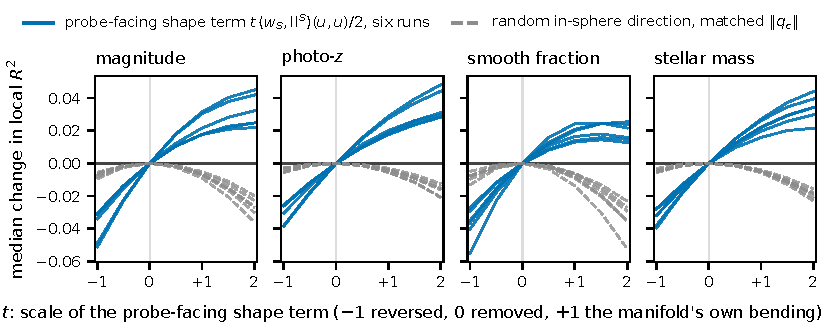
\includegraphics[width=\textwidth]{figures/fig1_intervention.pdf}
\caption{Bending toward the label helps, bending away hurts. At each of 512 anchors the readout's in-sphere shape quadratic $\tfrac t2\langle w_S,\mathrm{II}^S\rangle(u,u)$ is scaled by $t$ in a local second-order surrogate at a fixed manifold; lines are the median over anchors of the change in local $R^2$ relative to shape-flat ($t=0$). $t=1$ is the manifold's own bending seen from the readout's normal direction, $t=-1$ its reversal. Blue: the decoder's shape term, one line per run (five encoders at $d=16$, ViT-B also at $d=20$). Grey dashed: a random in-sphere normal direction with matched quadratic amplitude $\norm{q_c}$. Fractions of anchors helped and hurt, and sign tests on non-overlapping anchors, in Appendix~D.}
\label{fig:main}
\end{figure}

\paragraph{Galaxies.}
We estimate $\operatorname{Hess}_M y$ at each
anchor by fitting a least-squares quadratic
to the labels of its 2{,}048 neighbours in
tangent-projected coordinates
$u=g^{-1}J^\top(x-x_0)$. These decoder-based
Monge coordinates have vanishing Christoffel
symbols at the anchor, so the quadratic
coefficient estimates the covariant Hessian
in the small-neighbourhood limit. For
magnitude and redshift, the mismatch
$\|\Delta\|_g$ is negatively associated with
local $R^2$ ($-0.39$ to $-0.45$), while
alignment
$\cos_g(\operatorname{Hess}_M y,K)$
is positively associated with it
($+0.24$ to $+0.43$). These relationships
persist under cross-fitting (Appendix~B).
Smooth fraction exhibits weaker associations,
while stellar mass shows no significant
mismatch or alignment signal in this
experiment (Table~\ref{tab:real}; decoder
ablations, Appendix~A). Across five encoders, mismatch remains negatively associated with local accuracy for magnitude and redshift, while alignment is positive and significant for magnitude across all five and redshift across four (Appendix~C).

The shape term closely tracks the magnitude
of the total probe-facing curvature on
galaxies (rank correlation $0.96$--$0.99$),
but its association with local accuracy
varies across targets. This is consistent
with Eq.~\eqref{eq:resid}, where the shape
term's contribution to the quadratic
mismatch depends on both its magnitude and
its alignment with the remaining target
curvature. The sphere term is negatively
associated with local accuracy for all four
targets in the main ViT-B experiment,
although its association is sensitive to
probe regularization for some targets
(Appendix~E). Applying the same local
quadratic regression to the probe predictions
provides a decoder-independent estimate of
$K$, with median tensor cosine
$0.55$--$0.65$ relative to the
decoder-based estimate.

\paragraph{Relation to prior work.}
The identity in Eq.~\eqref{eq:hess} is
classical~\citep{milnor1963morse,chern1957total};
related work derives a curvature-dependent
normal weight for least-squares regression
on hypersurfaces~\citep{liu2023linear}
and documents the effects of curved
representations on linear
decoding~\citep{jurewicz2024irrational}.
Other approaches study manifold
capacity~\citep{chung2016linear,slatton2026linear},
representation flattening~\citep{psenka2024flattening},
curvature regularization~\citep{ma2023curvature},
latent geometry~\citep{kaufman2023latent},
local-regression bias~\citep{cheng2013local},
and geometric indicators of
generalization~\citep{chou2026diagnosing}.
Our contribution is to estimate the
pointwise probe-facing curvature tensor
on a learned manifold, compare it with
the target's intrinsic Hessian, and test
its contribution to local readout accuracy
through a controlled second-order intervention.

\paragraph{Bending toward helps, bending away hurts.}
To isolate the contribution of probe-facing
shape curvature, we intervene on the
in-sphere quadratic term of a local
second-order surrogate while keeping the
manifold, tangent readout, and sphere term
fixed. Each anchor's 2{,}048 neighbours
are scored by
$\hat y_t(u)=c+a^\top u+
\tfrac12K_{\mathrm{sph}}(u,u)+
\tfrac t2K_S(u,u)$,
where $a$ is the probe's tangent
differential, $K_S$ is estimated from the
decoder, and $c$ is refit for each $t$.
Here $t=1$ retains the estimated shape
quadratic of the original readout,
$t=-1$ reverses its sign, and $t=0$
removes it.

Under the isotropic Gaussian quadratic
model, $t=1$ improves upon $t=0$ iff
$2\langle R,K_S\rangle_g>\|K_S\|_g^2$.
On the actual neighbours, let $r_0$ be
the centred shape-flat residual and
$q_c$ the centred quadratic contribution
$\tfrac12K_S(u_i,u_i)$. After refitting
the intercept, the exact finite-sample
criterion is
$2\langle r_0,q_c\rangle>\|q_c\|^2$,
with optimum
$t^*=\langle r_0,q_c\rangle/\|q_c\|^2$
(Appendix~D).

Across five encoders and all four labels
(Figure~\ref{fig:main}), $t=1$ improves
local $R^2$ relative to the shape-flat
surrogate at 79--99\% of anchors, while
$t=-1$ reduces it at 97--100\%.
A random in-sphere normal direction with
matched centred quadratic amplitude shows
no comparable directional asymmetry and
is typically harmful under either sign
($t=1$ improves upon shape-flat at
22--36\% of anchors; Appendix~D).

Thus, the probe-selected shape quadratic
is locally error-reducing within the
second-order surrogate. Under the quadratic
Gaussian model, this is the signature of
bending toward the target's remaining
intrinsic curvature. This within-anchor
comparison differs from the cross-anchor
associations in Table~\ref{tab:real}
and can hold even where the latter show
no significant signal, as for stellar mass.
The optimum $t^*$ lies between 1.5 and
3.6 across runs, indicating that further
amplification of the shape term reduces
local surrogate error. 

\section{Discussion}

Our results identify a geometric source of local linear-probe error: the mismatch $\Delta=\operatorname{Hess}_M y-\langle w_N,\mathrm{II}\rangle$ between the target's intrinsic Hessian and the curvature induced by the probe. We estimate this mismatch using a decoder-based second fundamental form, validated on a synthetic surface and showing moderate agreement with a decoder-independent estimate on galaxy embeddings. Across five encoders, mismatch tracks local accuracy for magnitude and redshift, with weaker evidence for smooth fraction. A counterfactual intervention on the local second-order surrogate shows that the probe-selected shape term reduces error at most anchors, while reversing it generally increases error. Thus, manifold curvature can help rather than hinder linear decoding when it bends toward the target's curvature.

The mismatch can be estimated from labelled neighbours without knowing an object's target value, providing a local diagnostic of predictions that may warrant further scrutiny. It is not yet a calibrated per-object uncertainty estimate. For stellar mass, mismatch does not consistently track local accuracy despite the beneficial shape contribution, showing that a locally useful geometric effect need not explain variation in overall readout accuracy.

\emph{Limitations.}
We study one galaxy sample, four targets and five encoders. The label Hessian is estimated from finite neighbourhoods; its norm is reliably ranked (split-half $\rho=0.91$--$0.94$), but its direction is only moderately recovered (tensor cosine $0.19$--$0.35$). The synthetic surface does not independently corroborate the alignment association because its target has insufficient intrinsic curvature. The intervention modifies a local surrogate, not the encoder or manifold. Mismatch and alignment are the primary hypotheses; other analyses are exploratory. Overlapping neighbourhoods introduce anchor dependence that may affect permutation-test validity.

\bibliographystyle{unsrtnat}
{\small
\bibliography{references}
}

\appendix
% BEGIN APPENDIX AUTOGEN
\section*{Appendix A: decoder ablations}
Table~\ref{tab:ablate} repeats the four quantities of Tables~\ref{tab:real} and~\ref{tab:meancurv} at $d=16$ under the multi-scale density control for two further decoder initialisation seeds and for a decoder of width $400^3$ instead of $250^3$ (all fits reach variance explained 0.952). Every significant sign of the main table is retained.
\begin{table}[h]
\centering\footnotesize\setlength{\tabcolsep}{4pt}
\begin{tabular}{llcccc}
\toprule
label & quantity & seed 0 & seed 1 & seed 2 & $400^3$ \\
\midrule
mag\_r & shape & $+0.12$ & $+0.05^{*}$ & $+0.12$ & $+0.05^{*}$ \\
 & sphere & $-0.26$ & $-0.26$ & $-0.27$ & $-0.26$ \\
 & mismatch & $-0.39$ & $-0.35$ & $-0.34$ & $-0.34$ \\
 & alignment & $+0.35$ & $+0.31$ & $+0.37$ & $+0.41$ \\
\addlinespace[2pt]
photo\_z & shape & $-0.06^{*}$ & $-0.09^{*}$ & $-0.09$ & $-0.06^{*}$ \\
 & sphere & $-0.33$ & $-0.35$ & $-0.34$ & $-0.35$ \\
 & mismatch & $-0.45$ & $-0.43$ & $-0.42$ & $-0.41$ \\
 & alignment & $+0.26$ & $+0.24$ & $+0.25$ & $+0.25$ \\
\addlinespace[2pt]
smooth\_fraction & shape & $+0.07^{*}$ & $+0.20$ & $+0.15$ & $+0.10$ \\
 & sphere & $-0.13$ & $-0.15$ & $-0.14$ & $-0.11$ \\
 & mismatch & $-0.09^{*}$ & $-0.05^{*}$ & $-0.08^{*}$ & $-0.07^{*}$ \\
 & alignment & $+0.19$ & $+0.14$ & $+0.09$ & $+0.10$ \\
\addlinespace[2pt]
stellar\_mass & shape & $+0.00^{*}$ & $-0.06^{*}$ & $+0.05^{*}$ & $+0.09$ \\
 & sphere & $-0.35$ & $-0.35$ & $-0.35$ & $-0.35$ \\
 & mismatch & $-0.04^{*}$ & $+0.03^{*}$ & $+0.02^{*}$ & $+0.03^{*}$ \\
 & alignment & $+0.01^{*}$ & $-0.02^{*}$ & $+0.03^{*}$ & $-0.02^{*}$ \\
\addlinespace[2pt]
\bottomrule
\end{tabular}
\caption{Decoder ablations, $d=16$, 512 anchors, multi-scale density control. $^{*}$ not significant at 0.05.}
\label{tab:ablate}
\end{table}
\section*{Appendix B: sensitivity of the mismatch and sphere columns}
Cross-fitting: each 2{,}048-patch is split at random into halves; $\operatorname{Hess}_M y$ is fitted on one half and local $R^2$ scored on the other (both directions shown), so the Hessian estimate and the outcome share no rows. The split-half cosine between the two Hessian estimates is the reliability of the estimate. Weak ridge: the probe refit at $\alpha=1$ instead of 100 (global out-of-sample $R^2$ rises by 0.10 to 0.15), which substantially reduces the shrinkage of extreme predictions; the sphere term is recomputed from that probe.
\begin{table}[h]
\centering\footnotesize\setlength{\tabcolsep}{3.5pt}
\begin{tabular}{llcccccc}
\toprule
 & & \multicolumn{2}{c}{mismatch, cross-fit} & \multicolumn{2}{c}{alignment, cross-fit} & Hess.\ split cos & sphere, $\alpha=1$ \\
label & $d$ & fit A/score B & fit B/score A & fit A/score B & fit B/score A & p50 & (main: $\alpha=100$) \\
\midrule
mag\_r & 16 & $-0.38$ & $-0.34$ & $+0.33$ & $+0.31$ & +0.35 & $-0.21$ ($-0.26$) \\
mag\_r & 20 & $-0.43$ & $-0.40$ & $+0.39$ & $+0.37$ & +0.24 & $-0.22$ ($-0.26$) \\
photo\_z & 16 & $-0.42$ & $-0.36$ & $+0.23$ & $+0.20$ & +0.32 & $+0.05^{*}$ ($-0.33$) \\
photo\_z & 20 & $-0.42$ & $-0.42$ & $+0.22$ & $+0.22$ & +0.20 & $+0.03^{*}$ ($-0.36$) \\
smooth\_fraction & 16 & $-0.10$ & $-0.17$ & $+0.17$ & $+0.19$ & +0.33 & $-0.12$ ($-0.13$) \\
smooth\_fraction & 20 & $-0.15$ & $-0.21$ & $+0.05^{*}$ & $+0.03^{*}$ & +0.23 & $-0.13$ ($-0.15$) \\
stellar\_mass & 16 & $+0.01^{*}$ & $-0.04^{*}$ & $-0.03^{*}$ & $+0.06^{*}$ & +0.31 & $-0.02^{*}$ ($-0.35$) \\
stellar\_mass & 20 & $-0.06^{*}$ & $-0.07^{*}$ & $+0.01^{*}$ & $-0.00^{*}$ & +0.19 & $-0.02^{*}$ ($-0.35$) \\
\bottomrule
\end{tabular}
\caption{Cross-fitted mismatch and alignment partials (multi-scale control), split-half reliability of the label Hessian, and the sphere-term partial under a weak-ridge probe.}
\label{tab:sens}
\end{table}

\section*{Appendix C: Main and cross-encoder results}

\paragraph{Main results.}
Table~\ref{tab:real} reports the associations
between geometric mismatch, alignment and local
readout accuracy for ViT-B at $d=16$ and $d=20$.
Results use 512 anchors, $k=2{,}048$ neighbours
and the multi-scale density control.

\begin{table}[h]
\centering
\footnotesize
\setlength{\tabcolsep}{3.4pt}
\begin{tabular}{lcccc}
\toprule
 & \multicolumn{2}{c}{mismatch $\norm{\Delta}_g$}
 & \multicolumn{2}{c}{alignment $\cos_g(\operatorname{Hess}_M y, K)$} \\
label & $d{=}16$ & $d{=}20$ & $d{=}16$ & $d{=}20$ \\
\midrule
mag\_r & $-0.39$ & $-0.40$ & $+0.35$ & $+0.43$ \\
photo\_z & $-0.45$ & $-0.44$ & $+0.26$ & $+0.24$ \\
smooth\_fraction & $-0.09^{*}$ & $-0.17$ & $+0.19$ & $+0.07^{*}$ \\
stellar\_mass & $-0.04^{*}$ & $-0.09^{*}$ & $+0.01^{*}$ & $+0.02^{*}$ \\
\bottomrule
\end{tabular}
\caption{ViT-B: rank-partial Spearman correlations
with local $R^2$ under the multi-scale density
control. $^{*}$ Not significant at 0.05.
Shape, sphere and mean-curvature results
are reported in Appendix~E.}
\label{tab:real}
\end{table}

\paragraph{Across encoders.}
We repeat the geometric diagnostic at $d=16$
on the same 86{,}471 galaxies using four further
encoders from the Platonic Universe release:
DINOv3 ViT-B/16, CLIP ViT-B, ConvNeXt-B and
ViT-L (widths 768, 512, 1{,}024 and 1{,}024;
all unit-normalized).
A decoder of the same architecture and training
protocol is fitted per encoder (seed 0;
variance explained 0.966, 0.985, 0.965 and
0.968, respectively). All analyses use
512 anchors, $k=2{,}048$ and the multi-scale
density control.

For magnitude and redshift, mismatch is
negatively associated with local $R^2$
across all five encoders ($-0.32$ to $-0.61$;
cross-fitted $-0.28$ to $-0.62$).
Alignment is positive and significant for
magnitude across all five ($+0.13$ to $+0.53$)
and for redshift across four.
Shape-term associations vary by encoder and
target, while smooth fraction shows less
consistent mismatch and alignment signals.
For stellar mass, alignment is nonsignificant
across encoders and mismatch significant in
only one main comparison. Thus, the
cross-anchor mismatch association varies by
target, even where the shape term improves
the local surrogate.

Table~\ref{tab:xenc} reports the full
cross-encoder results, including global
out-of-sample probe $R^2$ in the first row
for each label. Table~\ref{tab:xencx}
reports cross-fitted mismatch and alignment
associations and split-half reliability of
the estimated label Hessian.

\begin{table}[h]
\centering
\footnotesize
\setlength{\tabcolsep}{4pt}
\begin{tabular}{llccccc}
\toprule
label & quantity & ViT-B & DINOv3 & CLIP-B & ConvNeXt-B & ViT-L \\
\midrule
mag\_r & global $R^2$ & 0.52 & 0.57 & 0.50 & 0.52 & 0.52 \\
 & shape & $+0.12$ & $-0.11$ & $+0.16$ & $+0.16$ & $-0.21$ \\
 & sphere & $-0.26$ & $-0.23$ & $-0.40$ & $-0.24$ & $-0.08^{*}$ \\
 & mismatch & $-0.39$ & $-0.57$ & $-0.34$ & $-0.32$ & $-0.44$ \\
 & alignment & $+0.35$ & $+0.53$ & $+0.32$ & $+0.21$ & $+0.13$ \\
\addlinespace[2pt]
photo\_z & global $R^2$ & 0.51 & 0.56 & 0.49 & 0.49 & 0.51 \\
 & shape & $-0.06^{*}$ & $-0.05^{*}$ & $-0.17$ & $+0.29$ & $-0.16$ \\
 & sphere & $-0.33$ & $-0.21$ & $-0.29$ & $-0.46$ & $-0.44$ \\
 & mismatch & $-0.45$ & $-0.61$ & $-0.45$ & $-0.48$ & $-0.46$ \\
 & alignment & $+0.26$ & $+0.33$ & $+0.06^{*}$ & $+0.22$ & $+0.14$ \\
\addlinespace[2pt]
smooth\_fraction & global $R^2$ & 0.53 & 0.59 & 0.49 & 0.56 & 0.55 \\
 & shape & $+0.07^{*}$ & $-0.08^{*}$ & $+0.20$ & $+0.24$ & $+0.06^{*}$ \\
 & sphere & $-0.13$ & $-0.06^{*}$ & $+0.05^{*}$ & $-0.15$ & $-0.11$ \\
 & mismatch & $-0.09^{*}$ & $-0.33$ & $-0.25$ & $-0.20$ & $-0.01^{*}$ \\
 & alignment & $+0.19$ & $-0.02^{*}$ & $+0.24$ & $+0.04^{*}$ & $+0.14$ \\
\addlinespace[2pt]
stellar\_mass & global $R^2$ & 0.48 & 0.54 & 0.50 & 0.49 & 0.49 \\
 & shape & $+0.00^{*}$ & $-0.15$ & $-0.10$ & $-0.11$ & $-0.13$ \\
 & sphere & $-0.35$ & $-0.26$ & $-0.38$ & $-0.40$ & $-0.38$ \\
 & mismatch & $-0.04^{*}$ & $+0.03^{*}$ & $-0.12$ & $-0.06^{*}$ & $-0.02^{*}$ \\
 & alignment & $+0.01^{*}$ & $-0.05^{*}$ & $-0.01^{*}$ & $+0.07^{*}$ & $-0.03^{*}$ \\
\addlinespace[2pt]
\bottomrule
\end{tabular}
\caption{Cross-encoder results at $d=16$:
global probe $R^2$ and rank-partial Spearman
correlations with local $R^2$ under the
multi-scale density control.
$^{*}$ Not significant at 0.05.}
\label{tab:xenc}
\end{table}

\begin{table}[h]
\centering
\footnotesize
\setlength{\tabcolsep}{3.5pt}
\begin{tabular}{llccccc}
\toprule
 & & \multicolumn{2}{c}{mismatch, cross-fit}
 & \multicolumn{2}{c}{alignment, cross-fit}
 & Hess.\ split cos \\
encoder & label & fit A/score B & fit B/score A
& fit A/score B & fit B/score A & p50 \\
\midrule
\addlinespace[2pt]
DINOv3 & mag\_r & $-0.60$ & $-0.62$ & $+0.50$ & $+0.50$ & +0.35 \\
 & photo\_z & $-0.56$ & $-0.59$ & $+0.28$ & $+0.27$ & +0.24 \\
 & smooth\_fraction & $-0.32$ & $-0.29$ & $-0.03^{*}$ & $-0.02^{*}$ & +0.31 \\
 & stellar\_mass & $+0.03^{*}$ & $+0.02^{*}$ & $-0.03^{*}$ & $-0.07^{*}$ & +0.22 \\
\addlinespace[2pt]
CLIP-B & mag\_r & $-0.28$ & $-0.35$ & $+0.28$ & $+0.29$ & +0.31 \\
 & photo\_z & $-0.41$ & $-0.40$ & $+0.08^{*}$ & $+0.06^{*}$ & +0.25 \\
 & smooth\_fraction & $-0.22$ & $-0.24$ & $+0.15$ & $+0.20$ & +0.28 \\
 & stellar\_mass & $-0.14$ & $-0.13$ & $-0.04^{*}$ & $+0.01^{*}$ & +0.19 \\
\addlinespace[2pt]
ConvNeXt-B & mag\_r & $-0.36$ & $-0.34$ & $+0.19$ & $+0.21$ & +0.29 \\
 & photo\_z & $-0.46$ & $-0.45$ & $+0.18$ & $+0.19$ & +0.30 \\
 & smooth\_fraction & $-0.15$ & $-0.19$ & $-0.02^{*}$ & $+0.03^{*}$ & +0.32 \\
 & stellar\_mass & $-0.05^{*}$ & $-0.01^{*}$ & $+0.14$ & $-0.03^{*}$ & +0.29 \\
\addlinespace[2pt]
ViT-L & mag\_r & $-0.46$ & $-0.49$ & $+0.09^{*}$ & $+0.15$ & +0.30 \\
 & photo\_z & $-0.44$ & $-0.42$ & $+0.09^{*}$ & $+0.13$ & +0.24 \\
 & smooth\_fraction & $-0.03^{*}$ & $-0.04^{*}$ & $+0.11$ & $+0.07^{*}$ & +0.30 \\
 & stellar\_mass & $-0.06^{*}$ & $+0.01^{*}$ & $-0.04^{*}$ & $-0.03^{*}$ & +0.21 \\
\addlinespace[2pt]
\bottomrule
\end{tabular}
\caption{Cross-fitted mismatch and alignment
partials under the multi-scale density
control, with median split-half tensor
cosine for the estimated label Hessian.
$^{*}$ Not significant at 0.05.}
\label{tab:xencx}
\end{table}
\section*{Appendix D: intervening on the readout's normal component}
The partials of Table~\ref{tab:real} compare anchors with one another and cannot say whether reversing the probe-facing shape term hurts relative to removing it, since no anchor is flat. Here we score a counterfactual local second-order surrogate of the readout at a fixed manifold. At each anchor the fitted ridge weight is split into tangent, radial and in-sphere normal parts $w = w_T + w_{\mathrm{rad}} + w_S$; we score the anchor's 2{,}048 neighbours by the data-side tangent-plus-sphere readout $(w_T + w_{\mathrm{rad}})\cdot x$ plus $t\,q$ with the local intercept refit, where $q = \tfrac12\langle w_S,\mathrm{II}^S\rangle(u,u)$ is the decoder's in-sphere second-order term in the anchor's chart coordinates: $t=1$ is the manifold's bending as seen in the readout's normal direction, $t=-1$ its sign reversal, $t=0$ shape-flat (the sphere term $-(w\!\cdot\!\hat x)g$ is kept in the base). Because the intercept is refit for every $t$, the local sum of squares is exactly $\mathrm{SSE}(t) = \norm{r_0 - t\,q_c}^2$ with $r_0$ the centred residual of the shape-flat predictor and $q_c = q - \bar q\mathbf 1$ the centred quadratic on the anchor's neighbours; hence $t^{*} = \langle r_0,q_c\rangle/\norm{q_c}^2$ and $t=1$ beats shape-flat iff $2\langle r_0,q_c\rangle > \norm{q_c}^2$. This is the finite-sample counterpart of the tensor-level condition $2\langle R,K_S\rangle_g > \norm{K_S}_g^2$ of Section~\ref{sec:theory}, not the same quantity: the tensor version needs the estimated label Hessian, the empirical one does not. Columns: fraction of anchors where $t=1$ beats shape-flat (help) and where $t=-1$ is worse than shape-flat (hurt), the median change in local $R^2$ at $t=\pm1$, the median $t^{*}$; then the same for a random in-sphere normal direction $v$ whose quadratic is rescaled to the same centred amplitude on the actual neighbours, $\norm{q_{v,c}} = \norm{q_c}$ (matching $\norm{v}$ to $\norm{w_S}$ instead leaves the contracted tensor at a fraction of the fitted one, since $\mathrm{II}^S$ spans at most $d(d+1)/2$ of the $\sim 750$ normal directions; matching $\norm{\langle v,\mathrm{II}^S\rangle}_g$ gives the same picture; Supplement 12). The anchors' neighbourhoods overlap (each point lies in about twelve of them), so the fractions are not counts of independent trials; a maximal set of anchors whose pairwise overlap is at most 5\% of $k$ has 19--21 members per run, on which $t=1$ beats shape-flat at 81--100\% (one-sided sign test $p \le 4\times 10^{-3}$ in every cell) and $t=-1$ is worse at 95--100\% ($p \le 3\times 10^{-5}$).
\begin{table}[h]
\centering\footnotesize\setlength{\tabcolsep}{3pt}
\begin{tabular}{llccccc|cccc}
\toprule
 & & \multicolumn{5}{c|}{decoder in-sphere shape term} & \multicolumn{4}{c}{random orientation, matched $\norm{q_c}$} \\
run & label & help & hurt & $\Delta R^2(+1)$ & $\Delta R^2(-1)$ & $t^{*}$ & help & hurt & $\Delta R^2(+1)$ & $\Delta R^2(-1)$ \\
\midrule
ViT-B, $d=16$ & mag\_r & 0.97 & 1.00 & $+0.030$ & $-0.051$ & 2.3 & 0.26 & 0.80 & $-0.009$ & $-0.009$ \\
 & photo\_z & 0.99 & 0.99 & $+0.028$ & $-0.038$ & 3.0 & 0.33 & 0.68 & $-0.005$ & $-0.006$ \\
 & smooth\_fraction & 0.90 & 1.00 & $+0.021$ & $-0.040$ & 1.7 & 0.24 & 0.78 & $-0.008$ & $-0.010$ \\
 & stellar\_mass & 0.96 & 0.99 & $+0.026$ & $-0.040$ & 2.6 & 0.29 & 0.70 & $-0.006$ & $-0.006$ \\
\addlinespace[2pt]
ViT-B, $d=20$ & mag\_r & 0.99 & 1.00 & $+0.031$ & $-0.049$ & 2.6 & 0.24 & 0.78 & $-0.007$ & $-0.008$ \\
 & photo\_z & 0.99 & 1.00 & $+0.029$ & $-0.038$ & 3.6 & 0.36 & 0.71 & $-0.004$ & $-0.005$ \\
 & smooth\_fraction & 0.90 & 1.00 & $+0.020$ & $-0.035$ & 1.9 & 0.22 & 0.77 & $-0.007$ & $-0.008$ \\
 & stellar\_mass & 0.97 & 1.00 & $+0.027$ & $-0.038$ & 3.1 & 0.32 & 0.72 & $-0.005$ & $-0.005$ \\
\addlinespace[2pt]
DINOv3, $d=16$ & mag\_r & 0.92 & 0.99 & $+0.018$ & $-0.031$ & 2.0 & 0.29 & 0.71 & $-0.007$ & $-0.006$ \\
 & photo\_z & 0.96 & 0.99 & $+0.020$ & $-0.030$ & 2.6 & 0.29 & 0.71 & $-0.006$ & $-0.004$ \\
 & smooth\_fraction & 0.93 & 1.00 & $+0.024$ & $-0.055$ & 1.5 & 0.22 & 0.78 & $-0.014$ & $-0.013$ \\
 & stellar\_mass & 0.95 & 1.00 & $+0.016$ & $-0.028$ & 2.1 & 0.26 & 0.74 & $-0.005$ & $-0.005$ \\
\addlinespace[2pt]
CLIP-B, $d=16$ & mag\_r & 0.95 & 0.99 & $+0.018$ & $-0.031$ & 2.2 & 0.30 & 0.68 & $-0.006$ & $-0.005$ \\
 & photo\_z & 0.99 & 1.00 & $+0.019$ & $-0.026$ & 3.4 & 0.36 & 0.64 & $-0.003$ & $-0.003$ \\
 & smooth\_fraction & 0.92 & 0.99 & $+0.014$ & $-0.027$ & 1.7 & 0.25 & 0.69 & $-0.006$ & $-0.005$ \\
 & stellar\_mass & 0.97 & 1.00 & $+0.020$ & $-0.028$ & 2.8 & 0.35 & 0.68 & $-0.004$ & $-0.005$ \\
\addlinespace[2pt]
ConvNeXt-B, $d=16$ & mag\_r & 0.92 & 1.00 & $+0.018$ & $-0.031$ & 2.0 & 0.26 & 0.73 & $-0.007$ & $-0.007$ \\
 & photo\_z & 0.99 & 1.00 & $+0.018$ & $-0.026$ & 2.9 & 0.28 & 0.64 & $-0.004$ & $-0.003$ \\
 & smooth\_fraction & 0.88 & 0.98 & $+0.016$ & $-0.036$ & 1.6 & 0.23 & 0.75 & $-0.009$ & $-0.008$ \\
 & stellar\_mass & 0.99 & 1.00 & $+0.022$ & $-0.032$ & 3.1 & 0.29 & 0.65 & $-0.005$ & $-0.003$ \\
\addlinespace[2pt]
ViT-L, $d=16$ & mag\_r & 0.96 & 0.99 & $+0.022$ & $-0.034$ & 2.6 & 0.32 & 0.74 & $-0.005$ & $-0.006$ \\
 & photo\_z & 0.97 & 0.99 & $+0.018$ & $-0.025$ & 3.2 & 0.34 & 0.67 & $-0.004$ & $-0.003$ \\
 & smooth\_fraction & 0.79 & 0.97 & $+0.013$ & $-0.029$ & 1.6 & 0.25 & 0.77 & $-0.006$ & $-0.008$ \\
 & stellar\_mass & 0.98 & 1.00 & $+0.022$ & $-0.032$ & 2.9 & 0.30 & 0.67 & $-0.004$ & $-0.004$ \\
\addlinespace[2pt]
\bottomrule
\end{tabular}
\caption{Counterfactual scaling of the in-sphere shape term in a local second-order surrogate of the readout, 512 anchors per run. The manifold's bending as seen in the readout's normal direction helps at a large majority of anchors, its sign reversal hurts at nearly every anchor, a random orientation of the same centred quadratic amplitude shows no such asymmetry and is typically harmful under either sign; $t^{*}>1$ throughout, consistent with the globally ridge-regularized probe under-using a locally beneficial term.}
\label{tab:cf}
\end{table}
% END APPENDIX AUTOGEN

% Appendix E is hand-written (not generated); numbers are the same record-verified values that stood in the main text until 2026-09-18.
\section*{Appendix E: the shape and sphere terms, and mean curvature}
\label{app:meancurv}
The mean-curvature vector of the decoder surface is $H = \operatorname{tr}_g \mathrm{II}$ (unnormalized trace; some authors divide by $d$). Alongside Eq.~\eqref{eq:hess}, $\Delta_M (w\!\cdot\! x) = \langle w, H\rangle$: the Laplacian of a linear readout sees only the trace of $\mathrm{II}$, its Hessian the whole tensor, so $\norm{H}$ need not track $\langle w_N,\mathrm{II}\rangle$. On the unit sphere the Euclidean mean-curvature vector of every $d$-submanifold has the universal radial component $-d\,\hat x$, which says nothing about shape; differentiating the projected decoder $F/\norm{F}$ splits $H = -d\,\hat x + \Htan$ exactly (radial part $-d$ to $10^{-14}$), and $\Htan$ is the non-radial mean-curvature component used below.

\emph{Validation surface.} At $D=768$ the in-sphere surface $G(z) = Q\,\mathrm{normalize}([\phi(z);\,0.8\,h(z);\,0\ldots])$ ($\phi$ inverse stereographic $\mathbb{R}^{16}\to S^{16}$, $h$ four Gaussian bumps, $Q$ a rotation) has closed-form curvature; the decoder's $\Htan$ gives rank 0.94 against the true $\norm{\Htan}$, direction cosine 0.999, magnitude ratio 1.00. Resampling this surface with weight $\norm{\Htan}^\gamma$ (Figure~\ref{fig:meancurv}a) moves the density-controlled $\norm{\Htan}$ partial against local $R^2$ from $-0.29$ to $+0.26$, while $\norm{\langle w_N,\mathrm{II}\rangle}_g$ holds at $-0.74$ to $-0.80$, dominated by the sphere term of Eq.~\eqref{eq:split}; the mismatch partial reproduces there, the alignment partial has no stable sign.

\emph{Galaxies: shape and sphere terms.} Table~\ref{tab:meancurv} gives the density-controlled partials of the two terms of Eq.~\eqref{eq:split} against local $R^2$ (Figure~\ref{fig:meancurv}b). The shape term dominates the probe-facing Hessian on galaxies (rank $0.96$--$0.99$ with $\norm{K}_g$) and is label-signed: positive for magnitude and smooth fraction, null to weakly negative for redshift, null for stellar mass. The sphere term is negative on every label and both $d$ ($-0.13$ to $-0.36$) under the $\alpha=100$ probe; with a weak-ridge probe ($\alpha=1$, Appendix~B) it stays negative for magnitude and smooth fraction ($-0.21$, $-0.12$) and vanishes for redshift and stellar mass, so part of it is ridge shrinkage of extreme predictions rather than geometry.

\emph{Galaxies: mean curvature.} The $\norm{\Htan}$ partial changes sign with the latent dimension for magnitude and is null for stellar mass. Across the five encoders of Appendix~C the quadratic-chart mean-bending trace has density-controlled associations with the magnitude probe's local $R^2$ of both signs ($-0.24$ to $+0.27$), as Eq.~\eqref{eq:hess} allows. Mean curvature, the scalar usually reported, keeps only the trace of $\mathrm{II}$ and fails accordingly: its association with readout accuracy changes sign with the sampling on the known surface and with the latent dimension and the encoder on galaxies.
\begin{table}[h]
\centering\footnotesize\setlength{\tabcolsep}{4pt}
\begin{tabular}{lcccccc}
\toprule
 & \multicolumn{2}{c}{shape $\norm{\langle w_S,\mathrm{II}^S\rangle}$} & \multicolumn{2}{c}{sphere $\sqrt d\,|\hat y-b_0|$} & \multicolumn{2}{c}{$\norm{\Htan}$} \\
label & $d{=}16$ & $d{=}20$ & 16 & 20 & 16 & 20 \\
\midrule
mag\_r & $+0.12$ & $+0.19$ & $-0.26$ & $-0.26$ & $+0.25$ & $-0.17$ \\
photo\_z & $-0.06^{*}$ & $-0.12$ & $-0.33$ & $-0.36$ & $+0.28$ & $+0.13$ \\
smooth\_fraction & $+0.07^{*}$ & $+0.16$ & $-0.13$ & $-0.15$ & $+0.21$ & $+0.15$ \\
stellar\_mass & $+0.00^{*}$ & $+0.03^{*}$ & $-0.35$ & $-0.35$ & $-0.02^{*}$ & $-0.00^{*}$ \\
\bottomrule
\end{tabular}
\caption{Galaxies, 512 anchors, $k=2{,}048$, multi-scale density control: rank-partial Spearman against local $R^2$ of the shape term, the sphere term and the scalar $\norm{\Htan}$. $^{*}$ not significant at 0.05.}
\label{tab:meancurv}
\end{table}
\begin{figure}[h]
\centering
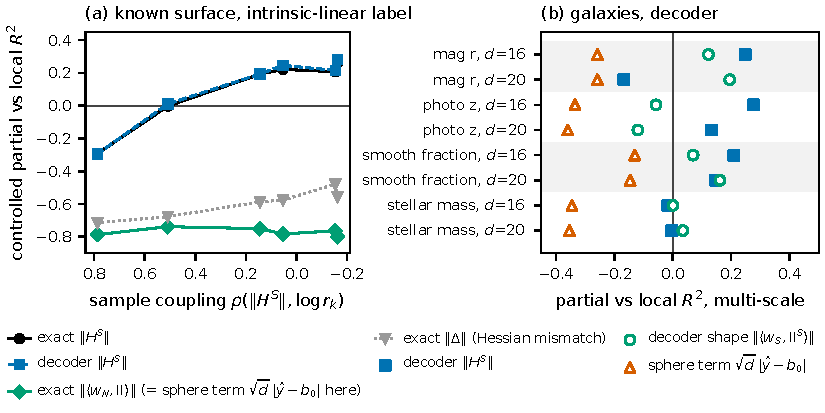
\includegraphics[width=0.85\textwidth]{figures/figF_mean_curvature.pdf}
\caption{(a) Known surface, linear label, exact geometry: three-control partial vs local $R^2$ as the density--curvature coupling is set by construction ($\gamma$ from $-1$ to $1$). (b) Galaxies, 512 anchors, $k=2{,}048$, multi-scale control: the decoder's $\norm{\Htan}$ (filled squares), shape term (open circles), sphere term (open triangles).}
\label{fig:meancurv}
\end{figure}
\end{document}
"` swaps Times for
% Computer Modern on machines without the Times metrics. CM is wider, so a 4-page fit here is
% conservative. Inactive on Overleaf and in the submitted build.
\ifdefined\LOCALFONTCHECK
  \renewcommand{\rmdefault}{cmr}\renewcommand{\sfdefault}{cmss}\renewcommand{\ttdefault}{cmtt}
\fi

\usepackage[utf8]{inputenc}
\usepackage[T1]{fontenc}
\usepackage{hyperref}
\usepackage{url}
\usepackage{booktabs}
\usepackage{amsmath,amssymb}
\usepackage{microtype}
\usepackage{xcolor}
\usepackage{graphicx}

\newcommand{\Htan}{H^{S}}
\newcommand{\norm}[1]{\lVert #1 \rVert}

\title{Linear Probes on Curved Latent Spaces}

\author{%
  Anonymous Author(s)\\
  Affiliation\\
  \texttt{email}
}

\begin{document}

\maketitle

\begin{abstract}
Linear probes are commonly used to evaluate learned representations and infer physical quantities for objects without direct measurements. However, their global predictive performance does not reveal where individual predictions are locally reliable or how the geometry of the learned representation contributes to their errors. Here we identify a geometric source of local readout error. Although a linear probe is affine in the ambient space, its restriction to a curved embedding manifold has a nonzero intrinsic Hessian given by $\langle w_N,\mathrm{II}\rangle$, the manifold's bending contracted with the probe's normal component. We turn this classical identity into a per-object measurement on galaxy embeddings from five encoders, using a decoder-based estimate of the second fundamental form validated on a synthetic surface of known curvature. Comparing this probe-facing curvature with the intrinsic Hessian of the physical target, we find that their mismatch predicts local readout accuracy for magnitude and photometric redshift, robustly under cross-fitting and across encoders. A counterfactual intervention on a local second-order surrogate further shows that reversing the probe-facing bending reduces local accuracy at nearly every anchor, whereas randomly oriented bending of matched strength does not exhibit the same asymmetry. The resulting tensor mismatch provides a geometric diagnostic of local linear-readout reliability and helps identify which physical quantities exhibit geometry-associated variation in prediction accuracy.
\end{abstract}

\section{Introduction}

Linear probes evaluate learned representations by measuring how accurately targets can be recovered from frozen embeddings~\citep{alain2017probes}. Their global performance, however, does not reveal where individual predictions are reliable or how representation geometry contributes to their errors. This matters in physical science, where probes infer quantities without direct measurements. For galaxy images, linear probes predict catalogue quantities such as magnitude, redshift and stellar mass~\citep{smith2024astropt}, but offer no local reliability diagnostic. We show that an ambient affine probe inherits curvature from the embedding manifold in its normal direction. The mismatch between this probe-facing curvature and the target's intrinsic Hessian captures a local source of prediction error.

We contribute (i) a decoder-based pointwise estimate of the second fundamental form, validated on a synthetic surface of known curvature; (ii) the application of the classical identity $\operatorname{Hess}_M(w\cdot x)=\langle w_N,\mathrm{II}\rangle$ to a fitted probe, with a residual expansion identifying its second-order approximation error; and (iii) evidence from 86{,}471 galaxies and five encoders that curvature mismatch predicts local readout accuracy for magnitude and redshift, supported by an intervention on a local second-order surrogate with a matched random-direction control.


\section{Pointwise curvature from a decoder}
\label{sec:instr}

\paragraph{Data.} 86{,}471 galaxies from the AstroPT galaxy set~\citep{smith2024astropt} with catalogue labels ($r$-band magnitude, photometric redshift, smooth fraction, stellar mass), embedded by a supervised ImageNet-21k ViT-B/16 (``ViT-B'' below) and by four further encoders (Section~\ref{sec:real}); embeddings from the Platonic Universe release~\citep{duraphe2025platonic}. We unit-normalize embeddings (data on $S^{D-1}$; $D=768$ for ViT-B).

\paragraph{Instrument.} Let $F:\mathbb{R}^d\to\mathbb{R}^{D}$ be the decoder of a plain auto-encoder (three hidden layers of width 250, SiLU), fit on 80\% of rows; we evaluate curvature on held-out rows. With $J = DF(z)$, metric $g = J^{\top}J$, normal projector $P_N = I - Jg^{-1}J^{\top}$ and second fundamental form $\mathrm{II} = P_N D^2F(z)$, all by automatic differentiation (cf.~\citep{lee2023curvature,acosta2023extrinsic}) at points where $DF$ has full column rank $d$. We differentiate the projected decoder $F/\norm{F}$, whose image lies on the unit sphere, so that $\mathrm{II}$ splits exactly into the sphere's universal radial part and an in-sphere shape part (Eq.~\eqref{eq:split}; Appendix~E).

\paragraph{Validation.} On a synthetic in-sphere surface at $D=768$ with closed-form $\mathrm{II}$ (Appendix~E), the decoder's estimate matches the true trace of $\mathrm{II}$ in direction (cosine 0.999), magnitude (ratio 1.00) and rank across points (0.94).

\section{What a linear readout sees on a curved manifold}
\label{sec:theory}


\paragraph{Notation.}
Let $M\subset\mathbb{R}^D$ be a $d$-dimensional
smooth embedded manifold, $d<D$, with anchor
$x_0\in M$. Let $J$ be an orthonormal tangent
frame at $x_0$ and $u$ normal coordinates in
this frame, so that locally
$x(u)=x_0+Ju+\tfrac12\mathrm{II}(u,u)
+O(\|u\|^3)$~\citep{lee2018riemannian}, where $\mathrm{II}$ is the
normal-valued second fundamental form. In
the numerical estimates, $J=DF$ is the
decoder Jacobian, with metric $g=J^\top J$,
and tangent-projected coordinates are used.
A probe weight decomposes as $w=w_T+w_N$
into tangent and normal components. On the
unit sphere, $\mathrm{II}=\mathrm{II}^S-g\,x$
separates the in-sphere shape from the
universal radial bending, and $w_S$ is
the component of $w_N$ orthogonal to $x$.
Let $y$ be a smooth target on $M$ and
$\hat y=w\cdot x+b_0$ a global affine probe.
Tensor norms and inner products use
$\langle A,B\rangle_g
=g^{ia}g^{jb}A_{ij}B_{ab}$.

Three facts follow. First, although the
probe is affine in the ambient space, its
restriction to $M$ is generally nonlinear
in intrinsic coordinates:
\begin{equation}
(d\hat y)_J=J^\top w,\qquad
\operatorname{Hess}_M\hat y
=\langle w_N,\mathrm{II}\rangle=:K.
\label{eq:hess}
\end{equation}
We call $K$ the probe-facing curvature.
Second, on the unit sphere it splits into
an in-sphere shape term and a radial term:
\begin{equation}
K=
\underbrace{\langle w_S,\mathrm{II}^S
\rangle}_{K_S}
+
\underbrace{[-(\hat y-b_0)g]}_{K_{\mathrm{sph}}}.
\label{eq:split}
\end{equation}
Thus, even an ambient affine readout
inherits intrinsic curvature from the
geometry of the representation.

Third, consider an isotropic Gaussian
patch $u\sim N(0,s^2I_d)$ in the
orthonormal tangent frame. For sufficiently
smooth embedding and target functions,
with controlled higher derivatives, let
$\bar c=\mathbb E_{\mathrm{patch}}[y-\hat y]$
be the patch-mean residual,
$\delta=(dy-d\hat y)_J$ the differential
mismatch, and
$\Delta=\operatorname{Hess}_M y-K$
the Hessian mismatch. Then
\begin{equation}
\begin{aligned}
\mathbb E_{\mathrm{patch}}
[(y-\hat y)^2]
={}&\bar c^{\,2}
+s^2\|\delta\|^2\\
&+\tfrac12s^4\|\Delta\|_g^2
+O(s^4\|\delta\|)+O(s^6).
\end{aligned}
\label{eq:resid}
\end{equation}
The Hessian mismatch therefore determines
the quadratic residual's contribution
to centered local error under this model.
Its contribution is smaller than at
$K=0$ iff
$2\langle\operatorname{Hess}_M y,K
\rangle_g>\|K\|_g^2$: the probe-facing
curvature must bend toward the target's
curvature, without overshooting it.
With the sphere term fixed, the
corresponding condition for the shape
term is
$2\langle R,K_S\rangle_g>\|K_S\|_g^2$,
where
$R=\operatorname{Hess}_M y-K_{\mathrm{sph}}$.
Section~\ref{sec:real} tests this
relationship. Since the quadratic
contribution scales as $s^4$, our
empirical analysis controls for
variation in local neighborhood scale.

\section{Probe-facing curvature: bending toward the label helps, bending away hurts}
\label{sec:real}

Statistic: five-fold out-of-fold ridge probe~\citep{alain2017probes} at the pre-registered $\alpha=100$ from embedding to label; local $R^2$ inside each of 512 anchors' 2{,}048-neighbourhoods; rank-partial Spearman against local $R^2$ with Freedman--Lane $p$-values~\citep{freedman1983permutation}, controlling for log patch radius, local label variance and count and, stronger, log radius at five scales.

\begin{figure}[t]
\centering
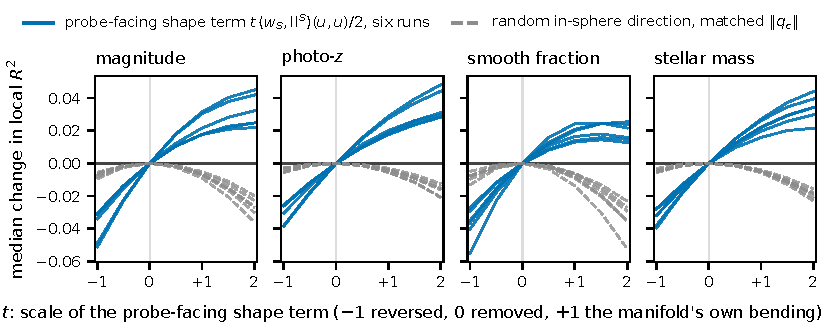
\includegraphics[width=\textwidth]{figures/fig1_intervention.pdf}
\caption{Bending toward the label helps, bending away hurts. At each of 512 anchors the readout's in-sphere shape quadratic $\tfrac t2\langle w_S,\mathrm{II}^S\rangle(u,u)$ is scaled by $t$ in a local second-order surrogate at a fixed manifold; lines are the median over anchors of the change in local $R^2$ relative to shape-flat ($t=0$). $t=1$ is the manifold's own bending seen from the readout's normal direction, $t=-1$ its reversal. Blue: the decoder's shape term, one line per run (five encoders at $d=16$, ViT-B also at $d=20$). Grey dashed: a random in-sphere normal direction with matched quadratic amplitude $\norm{q_c}$. Fractions of anchors helped and hurt, and sign tests on non-overlapping anchors, in Appendix~D.}
\label{fig:main}
\end{figure}

\paragraph{Galaxies.}
We estimate $\operatorname{Hess}_M y$ at each
anchor by fitting a least-squares quadratic
to the labels of its 2{,}048 neighbours in
tangent-projected coordinates
$u=g^{-1}J^\top(x-x_0)$. These decoder-based
Monge coordinates have vanishing Christoffel
symbols at the anchor, so the quadratic
coefficient estimates the covariant Hessian
in the small-neighbourhood limit. For
magnitude and redshift, the mismatch
$\|\Delta\|_g$ is negatively associated with
local $R^2$ ($-0.39$ to $-0.45$), while
alignment
$\cos_g(\operatorname{Hess}_M y,K)$
is positively associated with it
($+0.24$ to $+0.43$). These relationships
persist under cross-fitting (Appendix~B).
Smooth fraction exhibits weaker associations,
while stellar mass shows no significant
mismatch or alignment signal in this
experiment (Table~\ref{tab:real}; decoder
ablations, Appendix~A). Across five encoders, mismatch remains negatively associated with local accuracy for magnitude and redshift, while alignment is positive and significant for magnitude across all five and redshift across four (Appendix~C).

The shape term closely tracks the magnitude
of the total probe-facing curvature on
galaxies (rank correlation $0.96$--$0.99$),
but its association with local accuracy
varies across targets. This is consistent
with Eq.~\eqref{eq:resid}, where the shape
term's contribution to the quadratic
mismatch depends on both its magnitude and
its alignment with the remaining target
curvature. The sphere term is negatively
associated with local accuracy for all four
targets in the main ViT-B experiment,
although its association is sensitive to
probe regularization for some targets
(Appendix~E). Applying the same local
quadratic regression to the probe predictions
provides a decoder-independent estimate of
$K$, with median tensor cosine
$0.55$--$0.65$ relative to the
decoder-based estimate.

\paragraph{Relation to prior work.}
The identity in Eq.~\eqref{eq:hess} is
classical~\citep{milnor1963morse,chern1957total};
related work derives a curvature-dependent
normal weight for least-squares regression
on hypersurfaces~\citep{liu2023linear}
and documents the effects of curved
representations on linear
decoding~\citep{jurewicz2024irrational}.
Other approaches study manifold
capacity~\citep{chung2016linear,slatton2026linear},
representation flattening~\citep{psenka2024flattening},
curvature regularization~\citep{ma2023curvature},
latent geometry~\citep{kaufman2023latent},
local-regression bias~\citep{cheng2013local},
and geometric indicators of
generalization~\citep{chou2026diagnosing}.
Our contribution is to estimate the
pointwise probe-facing curvature tensor
on a learned manifold, compare it with
the target's intrinsic Hessian, and test
its contribution to local readout accuracy
through a controlled second-order intervention.

\paragraph{Bending toward helps, bending away hurts.}
To isolate the contribution of probe-facing
shape curvature, we intervene on the
in-sphere quadratic term of a local
second-order surrogate while keeping the
manifold, tangent readout, and sphere term
fixed. Each anchor's 2{,}048 neighbours
are scored by
$\hat y_t(u)=c+a^\top u+
\tfrac12K_{\mathrm{sph}}(u,u)+
\tfrac t2K_S(u,u)$,
where $a$ is the probe's tangent
differential, $K_S$ is estimated from the
decoder, and $c$ is refit for each $t$.
Here $t=1$ retains the estimated shape
quadratic of the original readout,
$t=-1$ reverses its sign, and $t=0$
removes it.

Under the isotropic Gaussian quadratic
model, $t=1$ improves upon $t=0$ iff
$2\langle R,K_S\rangle_g>\|K_S\|_g^2$.
On the actual neighbours, let $r_0$ be
the centred shape-flat residual and
$q_c$ the centred quadratic contribution
$\tfrac12K_S(u_i,u_i)$. After refitting
the intercept, the exact finite-sample
criterion is
$2\langle r_0,q_c\rangle>\|q_c\|^2$,
with optimum
$t^*=\langle r_0,q_c\rangle/\|q_c\|^2$
(Appendix~D).

Across five encoders and all four labels
(Figure~\ref{fig:main}), $t=1$ improves
local $R^2$ relative to the shape-flat
surrogate at 79--99\% of anchors, while
$t=-1$ reduces it at 97--100\%.
A random in-sphere normal direction with
matched centred quadratic amplitude shows
no comparable directional asymmetry and
is typically harmful under either sign
($t=1$ improves upon shape-flat at
22--36\% of anchors; Appendix~D).

Thus, the probe-selected shape quadratic
is locally error-reducing within the
second-order surrogate. Under the quadratic
Gaussian model, this is the signature of
bending toward the target's remaining
intrinsic curvature. This within-anchor
comparison differs from the cross-anchor
associations in Table~\ref{tab:real}
and can hold even where the latter show
no significant signal, as for stellar mass.
The optimum $t^*$ lies between 1.5 and
3.6 across runs, indicating that further
amplification of the shape term reduces
local surrogate error. 

\section{Discussion}

Our results identify a geometric source of local linear-probe error: the mismatch $\Delta=\operatorname{Hess}_M y-\langle w_N,\mathrm{II}\rangle$ between the target's intrinsic Hessian and the curvature induced by the probe. We estimate this mismatch using a decoder-based second fundamental form, validated on a synthetic surface and showing moderate agreement with a decoder-independent estimate on galaxy embeddings. Across five encoders, mismatch tracks local accuracy for magnitude and redshift, with weaker evidence for smooth fraction. A counterfactual intervention on the local second-order surrogate shows that the probe-selected shape term reduces error at most anchors, while reversing it generally increases error. Thus, manifold curvature can help rather than hinder linear decoding when it bends toward the target's curvature.

The mismatch can be estimated from labelled neighbours without knowing an object's target value, providing a local diagnostic of predictions that may warrant further scrutiny. It is not yet a calibrated per-object uncertainty estimate. For stellar mass, mismatch does not consistently track local accuracy despite the beneficial shape contribution, showing that a locally useful geometric effect need not explain variation in overall readout accuracy.

\emph{Limitations.}
We study one galaxy sample, four targets and five encoders. The label Hessian is estimated from finite neighbourhoods; its norm is reliably ranked (split-half $\rho=0.91$--$0.94$), but its direction is only moderately recovered (tensor cosine $0.19$--$0.35$). The synthetic surface does not independently corroborate the alignment association because its target has insufficient intrinsic curvature. The intervention modifies a local surrogate, not the encoder or manifold. Mismatch and alignment are the primary hypotheses; other analyses are exploratory. Overlapping neighbourhoods introduce anchor dependence that may affect permutation-test validity.

\bibliographystyle{unsrtnat}
{\small
\bibliography{references}
}

\appendix
% BEGIN APPENDIX AUTOGEN
\section*{Appendix A: decoder ablations}
Table~\ref{tab:ablate} repeats the four quantities of Tables~\ref{tab:real} and~\ref{tab:meancurv} at $d=16$ under the multi-scale density control for two further decoder initialisation seeds and for a decoder of width $400^3$ instead of $250^3$ (all fits reach variance explained 0.952). Every significant sign of the main table is retained.
\begin{table}[h]
\centering\footnotesize\setlength{\tabcolsep}{4pt}
\begin{tabular}{llcccc}
\toprule
label & quantity & seed 0 & seed 1 & seed 2 & $400^3$ \\
\midrule
mag\_r & shape & $+0.12$ & $+0.05^{*}$ & $+0.12$ & $+0.05^{*}$ \\
 & sphere & $-0.26$ & $-0.26$ & $-0.27$ & $-0.26$ \\
 & mismatch & $-0.39$ & $-0.35$ & $-0.34$ & $-0.34$ \\
 & alignment & $+0.35$ & $+0.31$ & $+0.37$ & $+0.41$ \\
\addlinespace[2pt]
photo\_z & shape & $-0.06^{*}$ & $-0.09^{*}$ & $-0.09$ & $-0.06^{*}$ \\
 & sphere & $-0.33$ & $-0.35$ & $-0.34$ & $-0.35$ \\
 & mismatch & $-0.45$ & $-0.43$ & $-0.42$ & $-0.41$ \\
 & alignment & $+0.26$ & $+0.24$ & $+0.25$ & $+0.25$ \\
\addlinespace[2pt]
smooth\_fraction & shape & $+0.07^{*}$ & $+0.20$ & $+0.15$ & $+0.10$ \\
 & sphere & $-0.13$ & $-0.15$ & $-0.14$ & $-0.11$ \\
 & mismatch & $-0.09^{*}$ & $-0.05^{*}$ & $-0.08^{*}$ & $-0.07^{*}$ \\
 & alignment & $+0.19$ & $+0.14$ & $+0.09$ & $+0.10$ \\
\addlinespace[2pt]
stellar\_mass & shape & $+0.00^{*}$ & $-0.06^{*}$ & $+0.05^{*}$ & $+0.09$ \\
 & sphere & $-0.35$ & $-0.35$ & $-0.35$ & $-0.35$ \\
 & mismatch & $-0.04^{*}$ & $+0.03^{*}$ & $+0.02^{*}$ & $+0.03^{*}$ \\
 & alignment & $+0.01^{*}$ & $-0.02^{*}$ & $+0.03^{*}$ & $-0.02^{*}$ \\
\addlinespace[2pt]
\bottomrule
\end{tabular}
\caption{Decoder ablations, $d=16$, 512 anchors, multi-scale density control. $^{*}$ not significant at 0.05.}
\label{tab:ablate}
\end{table}
\section*{Appendix B: sensitivity of the mismatch and sphere columns}
Cross-fitting: each 2{,}048-patch is split at random into halves; $\operatorname{Hess}_M y$ is fitted on one half and local $R^2$ scored on the other (both directions shown), so the Hessian estimate and the outcome share no rows. The split-half cosine between the two Hessian estimates is the reliability of the estimate. Weak ridge: the probe refit at $\alpha=1$ instead of 100 (global out-of-sample $R^2$ rises by 0.10 to 0.15), which substantially reduces the shrinkage of extreme predictions; the sphere term is recomputed from that probe.
\begin{table}[h]
\centering\footnotesize\setlength{\tabcolsep}{3.5pt}
\begin{tabular}{llcccccc}
\toprule
 & & \multicolumn{2}{c}{mismatch, cross-fit} & \multicolumn{2}{c}{alignment, cross-fit} & Hess.\ split cos & sphere, $\alpha=1$ \\
label & $d$ & fit A/score B & fit B/score A & fit A/score B & fit B/score A & p50 & (main: $\alpha=100$) \\
\midrule
mag\_r & 16 & $-0.38$ & $-0.34$ & $+0.33$ & $+0.31$ & +0.35 & $-0.21$ ($-0.26$) \\
mag\_r & 20 & $-0.43$ & $-0.40$ & $+0.39$ & $+0.37$ & +0.24 & $-0.22$ ($-0.26$) \\
photo\_z & 16 & $-0.42$ & $-0.36$ & $+0.23$ & $+0.20$ & +0.32 & $+0.05^{*}$ ($-0.33$) \\
photo\_z & 20 & $-0.42$ & $-0.42$ & $+0.22$ & $+0.22$ & +0.20 & $+0.03^{*}$ ($-0.36$) \\
smooth\_fraction & 16 & $-0.10$ & $-0.17$ & $+0.17$ & $+0.19$ & +0.33 & $-0.12$ ($-0.13$) \\
smooth\_fraction & 20 & $-0.15$ & $-0.21$ & $+0.05^{*}$ & $+0.03^{*}$ & +0.23 & $-0.13$ ($-0.15$) \\
stellar\_mass & 16 & $+0.01^{*}$ & $-0.04^{*}$ & $-0.03^{*}$ & $+0.06^{*}$ & +0.31 & $-0.02^{*}$ ($-0.35$) \\
stellar\_mass & 20 & $-0.06^{*}$ & $-0.07^{*}$ & $+0.01^{*}$ & $-0.00^{*}$ & +0.19 & $-0.02^{*}$ ($-0.35$) \\
\bottomrule
\end{tabular}
\caption{Cross-fitted mismatch and alignment partials (multi-scale control), split-half reliability of the label Hessian, and the sphere-term partial under a weak-ridge probe.}
\label{tab:sens}
\end{table}

\section*{Appendix C: Main and cross-encoder results}

\paragraph{Main results.}
Table~\ref{tab:real} reports the associations
between geometric mismatch, alignment and local
readout accuracy for ViT-B at $d=16$ and $d=20$.
Results use 512 anchors, $k=2{,}048$ neighbours
and the multi-scale density control.

\begin{table}[h]
\centering
\footnotesize
\setlength{\tabcolsep}{3.4pt}
\begin{tabular}{lcccc}
\toprule
 & \multicolumn{2}{c}{mismatch $\norm{\Delta}_g$}
 & \multicolumn{2}{c}{alignment $\cos_g(\operatorname{Hess}_M y, K)$} \\
label & $d{=}16$ & $d{=}20$ & $d{=}16$ & $d{=}20$ \\
\midrule
mag\_r & $-0.39$ & $-0.40$ & $+0.35$ & $+0.43$ \\
photo\_z & $-0.45$ & $-0.44$ & $+0.26$ & $+0.24$ \\
smooth\_fraction & $-0.09^{*}$ & $-0.17$ & $+0.19$ & $+0.07^{*}$ \\
stellar\_mass & $-0.04^{*}$ & $-0.09^{*}$ & $+0.01^{*}$ & $+0.02^{*}$ \\
\bottomrule
\end{tabular}
\caption{ViT-B: rank-partial Spearman correlations
with local $R^2$ under the multi-scale density
control. $^{*}$ Not significant at 0.05.
Shape, sphere and mean-curvature results
are reported in Appendix~E.}
\label{tab:real}
\end{table}

\paragraph{Across encoders.}
We repeat the geometric diagnostic at $d=16$
on the same 86{,}471 galaxies using four further
encoders from the Platonic Universe release:
DINOv3 ViT-B/16, CLIP ViT-B, ConvNeXt-B and
ViT-L (widths 768, 512, 1{,}024 and 1{,}024;
all unit-normalized).
A decoder of the same architecture and training
protocol is fitted per encoder (seed 0;
variance explained 0.966, 0.985, 0.965 and
0.968, respectively). All analyses use
512 anchors, $k=2{,}048$ and the multi-scale
density control.

For magnitude and redshift, mismatch is
negatively associated with local $R^2$
across all five encoders ($-0.32$ to $-0.61$;
cross-fitted $-0.28$ to $-0.62$).
Alignment is positive and significant for
magnitude across all five ($+0.13$ to $+0.53$)
and for redshift across four.
Shape-term associations vary by encoder and
target, while smooth fraction shows less
consistent mismatch and alignment signals.
For stellar mass, alignment is nonsignificant
across encoders and mismatch significant in
only one main comparison. Thus, the
cross-anchor mismatch association varies by
target, even where the shape term improves
the local surrogate.

Table~\ref{tab:xenc} reports the full
cross-encoder results, including global
out-of-sample probe $R^2$ in the first row
for each label. Table~\ref{tab:xencx}
reports cross-fitted mismatch and alignment
associations and split-half reliability of
the estimated label Hessian.

\begin{table}[h]
\centering
\footnotesize
\setlength{\tabcolsep}{4pt}
\begin{tabular}{llccccc}
\toprule
label & quantity & ViT-B & DINOv3 & CLIP-B & ConvNeXt-B & ViT-L \\
\midrule
mag\_r & global $R^2$ & 0.52 & 0.57 & 0.50 & 0.52 & 0.52 \\
 & shape & $+0.12$ & $-0.11$ & $+0.16$ & $+0.16$ & $-0.21$ \\
 & sphere & $-0.26$ & $-0.23$ & $-0.40$ & $-0.24$ & $-0.08^{*}$ \\
 & mismatch & $-0.39$ & $-0.57$ & $-0.34$ & $-0.32$ & $-0.44$ \\
 & alignment & $+0.35$ & $+0.53$ & $+0.32$ & $+0.21$ & $+0.13$ \\
\addlinespace[2pt]
photo\_z & global $R^2$ & 0.51 & 0.56 & 0.49 & 0.49 & 0.51 \\
 & shape & $-0.06^{*}$ & $-0.05^{*}$ & $-0.17$ & $+0.29$ & $-0.16$ \\
 & sphere & $-0.33$ & $-0.21$ & $-0.29$ & $-0.46$ & $-0.44$ \\
 & mismatch & $-0.45$ & $-0.61$ & $-0.45$ & $-0.48$ & $-0.46$ \\
 & alignment & $+0.26$ & $+0.33$ & $+0.06^{*}$ & $+0.22$ & $+0.14$ \\
\addlinespace[2pt]
smooth\_fraction & global $R^2$ & 0.53 & 0.59 & 0.49 & 0.56 & 0.55 \\
 & shape & $+0.07^{*}$ & $-0.08^{*}$ & $+0.20$ & $+0.24$ & $+0.06^{*}$ \\
 & sphere & $-0.13$ & $-0.06^{*}$ & $+0.05^{*}$ & $-0.15$ & $-0.11$ \\
 & mismatch & $-0.09^{*}$ & $-0.33$ & $-0.25$ & $-0.20$ & $-0.01^{*}$ \\
 & alignment & $+0.19$ & $-0.02^{*}$ & $+0.24$ & $+0.04^{*}$ & $+0.14$ \\
\addlinespace[2pt]
stellar\_mass & global $R^2$ & 0.48 & 0.54 & 0.50 & 0.49 & 0.49 \\
 & shape & $+0.00^{*}$ & $-0.15$ & $-0.10$ & $-0.11$ & $-0.13$ \\
 & sphere & $-0.35$ & $-0.26$ & $-0.38$ & $-0.40$ & $-0.38$ \\
 & mismatch & $-0.04^{*}$ & $+0.03^{*}$ & $-0.12$ & $-0.06^{*}$ & $-0.02^{*}$ \\
 & alignment & $+0.01^{*}$ & $-0.05^{*}$ & $-0.01^{*}$ & $+0.07^{*}$ & $-0.03^{*}$ \\
\addlinespace[2pt]
\bottomrule
\end{tabular}
\caption{Cross-encoder results at $d=16$:
global probe $R^2$ and rank-partial Spearman
correlations with local $R^2$ under the
multi-scale density control.
$^{*}$ Not significant at 0.05.}
\label{tab:xenc}
\end{table}

\begin{table}[h]
\centering
\footnotesize
\setlength{\tabcolsep}{3.5pt}
\begin{tabular}{llccccc}
\toprule
 & & \multicolumn{2}{c}{mismatch, cross-fit}
 & \multicolumn{2}{c}{alignment, cross-fit}
 & Hess.\ split cos \\
encoder & label & fit A/score B & fit B/score A
& fit A/score B & fit B/score A & p50 \\
\midrule
\addlinespace[2pt]
DINOv3 & mag\_r & $-0.60$ & $-0.62$ & $+0.50$ & $+0.50$ & +0.35 \\
 & photo\_z & $-0.56$ & $-0.59$ & $+0.28$ & $+0.27$ & +0.24 \\
 & smooth\_fraction & $-0.32$ & $-0.29$ & $-0.03^{*}$ & $-0.02^{*}$ & +0.31 \\
 & stellar\_mass & $+0.03^{*}$ & $+0.02^{*}$ & $-0.03^{*}$ & $-0.07^{*}$ & +0.22 \\
\addlinespace[2pt]
CLIP-B & mag\_r & $-0.28$ & $-0.35$ & $+0.28$ & $+0.29$ & +0.31 \\
 & photo\_z & $-0.41$ & $-0.40$ & $+0.08^{*}$ & $+0.06^{*}$ & +0.25 \\
 & smooth\_fraction & $-0.22$ & $-0.24$ & $+0.15$ & $+0.20$ & +0.28 \\
 & stellar\_mass & $-0.14$ & $-0.13$ & $-0.04^{*}$ & $+0.01^{*}$ & +0.19 \\
\addlinespace[2pt]
ConvNeXt-B & mag\_r & $-0.36$ & $-0.34$ & $+0.19$ & $+0.21$ & +0.29 \\
 & photo\_z & $-0.46$ & $-0.45$ & $+0.18$ & $+0.19$ & +0.30 \\
 & smooth\_fraction & $-0.15$ & $-0.19$ & $-0.02^{*}$ & $+0.03^{*}$ & +0.32 \\
 & stellar\_mass & $-0.05^{*}$ & $-0.01^{*}$ & $+0.14$ & $-0.03^{*}$ & +0.29 \\
\addlinespace[2pt]
ViT-L & mag\_r & $-0.46$ & $-0.49$ & $+0.09^{*}$ & $+0.15$ & +0.30 \\
 & photo\_z & $-0.44$ & $-0.42$ & $+0.09^{*}$ & $+0.13$ & +0.24 \\
 & smooth\_fraction & $-0.03^{*}$ & $-0.04^{*}$ & $+0.11$ & $+0.07^{*}$ & +0.30 \\
 & stellar\_mass & $-0.06^{*}$ & $+0.01^{*}$ & $-0.04^{*}$ & $-0.03^{*}$ & +0.21 \\
\addlinespace[2pt]
\bottomrule
\end{tabular}
\caption{Cross-fitted mismatch and alignment
partials under the multi-scale density
control, with median split-half tensor
cosine for the estimated label Hessian.
$^{*}$ Not significant at 0.05.}
\label{tab:xencx}
\end{table}
\section*{Appendix D: intervening on the readout's normal component}
The partials of Table~\ref{tab:real} compare anchors with one another and cannot say whether reversing the probe-facing shape term hurts relative to removing it, since no anchor is flat. Here we score a counterfactual local second-order surrogate of the readout at a fixed manifold. At each anchor the fitted ridge weight is split into tangent, radial and in-sphere normal parts $w = w_T + w_{\mathrm{rad}} + w_S$; we score the anchor's 2{,}048 neighbours by the data-side tangent-plus-sphere readout $(w_T + w_{\mathrm{rad}})\cdot x$ plus $t\,q$ with the local intercept refit, where $q = \tfrac12\langle w_S,\mathrm{II}^S\rangle(u,u)$ is the decoder's in-sphere second-order term in the anchor's chart coordinates: $t=1$ is the manifold's bending as seen in the readout's normal direction, $t=-1$ its sign reversal, $t=0$ shape-flat (the sphere term $-(w\!\cdot\!\hat x)g$ is kept in the base). Because the intercept is refit for every $t$, the local sum of squares is exactly $\mathrm{SSE}(t) = \norm{r_0 - t\,q_c}^2$ with $r_0$ the centred residual of the shape-flat predictor and $q_c = q - \bar q\mathbf 1$ the centred quadratic on the anchor's neighbours; hence $t^{*} = \langle r_0,q_c\rangle/\norm{q_c}^2$ and $t=1$ beats shape-flat iff $2\langle r_0,q_c\rangle > \norm{q_c}^2$. This is the finite-sample counterpart of the tensor-level condition $2\langle R,K_S\rangle_g > \norm{K_S}_g^2$ of Section~\ref{sec:theory}, not the same quantity: the tensor version needs the estimated label Hessian, the empirical one does not. Columns: fraction of anchors where $t=1$ beats shape-flat (help) and where $t=-1$ is worse than shape-flat (hurt), the median change in local $R^2$ at $t=\pm1$, the median $t^{*}$; then the same for a random in-sphere normal direction $v$ whose quadratic is rescaled to the same centred amplitude on the actual neighbours, $\norm{q_{v,c}} = \norm{q_c}$ (matching $\norm{v}$ to $\norm{w_S}$ instead leaves the contracted tensor at a fraction of the fitted one, since $\mathrm{II}^S$ spans at most $d(d+1)/2$ of the $\sim 750$ normal directions; matching $\norm{\langle v,\mathrm{II}^S\rangle}_g$ gives the same picture; Supplement 12). The anchors' neighbourhoods overlap (each point lies in about twelve of them), so the fractions are not counts of independent trials; a maximal set of anchors whose pairwise overlap is at most 5\% of $k$ has 19--21 members per run, on which $t=1$ beats shape-flat at 81--100\% (one-sided sign test $p \le 4\times 10^{-3}$ in every cell) and $t=-1$ is worse at 95--100\% ($p \le 3\times 10^{-5}$).
\begin{table}[h]
\centering\footnotesize\setlength{\tabcolsep}{3pt}
\begin{tabular}{llccccc|cccc}
\toprule
 & & \multicolumn{5}{c|}{decoder in-sphere shape term} & \multicolumn{4}{c}{random orientation, matched $\norm{q_c}$} \\
run & label & help & hurt & $\Delta R^2(+1)$ & $\Delta R^2(-1)$ & $t^{*}$ & help & hurt & $\Delta R^2(+1)$ & $\Delta R^2(-1)$ \\
\midrule
ViT-B, $d=16$ & mag\_r & 0.97 & 1.00 & $+0.030$ & $-0.051$ & 2.3 & 0.26 & 0.80 & $-0.009$ & $-0.009$ \\
 & photo\_z & 0.99 & 0.99 & $+0.028$ & $-0.038$ & 3.0 & 0.33 & 0.68 & $-0.005$ & $-0.006$ \\
 & smooth\_fraction & 0.90 & 1.00 & $+0.021$ & $-0.040$ & 1.7 & 0.24 & 0.78 & $-0.008$ & $-0.010$ \\
 & stellar\_mass & 0.96 & 0.99 & $+0.026$ & $-0.040$ & 2.6 & 0.29 & 0.70 & $-0.006$ & $-0.006$ \\
\addlinespace[2pt]
ViT-B, $d=20$ & mag\_r & 0.99 & 1.00 & $+0.031$ & $-0.049$ & 2.6 & 0.24 & 0.78 & $-0.007$ & $-0.008$ \\
 & photo\_z & 0.99 & 1.00 & $+0.029$ & $-0.038$ & 3.6 & 0.36 & 0.71 & $-0.004$ & $-0.005$ \\
 & smooth\_fraction & 0.90 & 1.00 & $+0.020$ & $-0.035$ & 1.9 & 0.22 & 0.77 & $-0.007$ & $-0.008$ \\
 & stellar\_mass & 0.97 & 1.00 & $+0.027$ & $-0.038$ & 3.1 & 0.32 & 0.72 & $-0.005$ & $-0.005$ \\
\addlinespace[2pt]
DINOv3, $d=16$ & mag\_r & 0.92 & 0.99 & $+0.018$ & $-0.031$ & 2.0 & 0.29 & 0.71 & $-0.007$ & $-0.006$ \\
 & photo\_z & 0.96 & 0.99 & $+0.020$ & $-0.030$ & 2.6 & 0.29 & 0.71 & $-0.006$ & $-0.004$ \\
 & smooth\_fraction & 0.93 & 1.00 & $+0.024$ & $-0.055$ & 1.5 & 0.22 & 0.78 & $-0.014$ & $-0.013$ \\
 & stellar\_mass & 0.95 & 1.00 & $+0.016$ & $-0.028$ & 2.1 & 0.26 & 0.74 & $-0.005$ & $-0.005$ \\
\addlinespace[2pt]
CLIP-B, $d=16$ & mag\_r & 0.95 & 0.99 & $+0.018$ & $-0.031$ & 2.2 & 0.30 & 0.68 & $-0.006$ & $-0.005$ \\
 & photo\_z & 0.99 & 1.00 & $+0.019$ & $-0.026$ & 3.4 & 0.36 & 0.64 & $-0.003$ & $-0.003$ \\
 & smooth\_fraction & 0.92 & 0.99 & $+0.014$ & $-0.027$ & 1.7 & 0.25 & 0.69 & $-0.006$ & $-0.005$ \\
 & stellar\_mass & 0.97 & 1.00 & $+0.020$ & $-0.028$ & 2.8 & 0.35 & 0.68 & $-0.004$ & $-0.005$ \\
\addlinespace[2pt]
ConvNeXt-B, $d=16$ & mag\_r & 0.92 & 1.00 & $+0.018$ & $-0.031$ & 2.0 & 0.26 & 0.73 & $-0.007$ & $-0.007$ \\
 & photo\_z & 0.99 & 1.00 & $+0.018$ & $-0.026$ & 2.9 & 0.28 & 0.64 & $-0.004$ & $-0.003$ \\
 & smooth\_fraction & 0.88 & 0.98 & $+0.016$ & $-0.036$ & 1.6 & 0.23 & 0.75 & $-0.009$ & $-0.008$ \\
 & stellar\_mass & 0.99 & 1.00 & $+0.022$ & $-0.032$ & 3.1 & 0.29 & 0.65 & $-0.005$ & $-0.003$ \\
\addlinespace[2pt]
ViT-L, $d=16$ & mag\_r & 0.96 & 0.99 & $+0.022$ & $-0.034$ & 2.6 & 0.32 & 0.74 & $-0.005$ & $-0.006$ \\
 & photo\_z & 0.97 & 0.99 & $+0.018$ & $-0.025$ & 3.2 & 0.34 & 0.67 & $-0.004$ & $-0.003$ \\
 & smooth\_fraction & 0.79 & 0.97 & $+0.013$ & $-0.029$ & 1.6 & 0.25 & 0.77 & $-0.006$ & $-0.008$ \\
 & stellar\_mass & 0.98 & 1.00 & $+0.022$ & $-0.032$ & 2.9 & 0.30 & 0.67 & $-0.004$ & $-0.004$ \\
\addlinespace[2pt]
\bottomrule
\end{tabular}
\caption{Counterfactual scaling of the in-sphere shape term in a local second-order surrogate of the readout, 512 anchors per run. The manifold's bending as seen in the readout's normal direction helps at a large majority of anchors, its sign reversal hurts at nearly every anchor, a random orientation of the same centred quadratic amplitude shows no such asymmetry and is typically harmful under either sign; $t^{*}>1$ throughout, consistent with the globally ridge-regularized probe under-using a locally beneficial term.}
\label{tab:cf}
\end{table}
% END APPENDIX AUTOGEN

% Appendix E is hand-written (not generated); numbers are the same record-verified values that stood in the main text until 2026-09-18.
\section*{Appendix E: the shape and sphere terms, and mean curvature}
\label{app:meancurv}
The mean-curvature vector of the decoder surface is $H = \operatorname{tr}_g \mathrm{II}$ (unnormalized trace; some authors divide by $d$). Alongside Eq.~\eqref{eq:hess}, $\Delta_M (w\!\cdot\! x) = \langle w, H\rangle$: the Laplacian of a linear readout sees only the trace of $\mathrm{II}$, its Hessian the whole tensor, so $\norm{H}$ need not track $\langle w_N,\mathrm{II}\rangle$. On the unit sphere the Euclidean mean-curvature vector of every $d$-submanifold has the universal radial component $-d\,\hat x$, which says nothing about shape; differentiating the projected decoder $F/\norm{F}$ splits $H = -d\,\hat x + \Htan$ exactly (radial part $-d$ to $10^{-14}$), and $\Htan$ is the non-radial mean-curvature component used below.

\emph{Validation surface.} At $D=768$ the in-sphere surface $G(z) = Q\,\mathrm{normalize}([\phi(z);\,0.8\,h(z);\,0\ldots])$ ($\phi$ inverse stereographic $\mathbb{R}^{16}\to S^{16}$, $h$ four Gaussian bumps, $Q$ a rotation) has closed-form curvature; the decoder's $\Htan$ gives rank 0.94 against the true $\norm{\Htan}$, direction cosine 0.999, magnitude ratio 1.00. Resampling this surface with weight $\norm{\Htan}^\gamma$ (Figure~\ref{fig:meancurv}a) moves the density-controlled $\norm{\Htan}$ partial against local $R^2$ from $-0.29$ to $+0.26$, while $\norm{\langle w_N,\mathrm{II}\rangle}_g$ holds at $-0.74$ to $-0.80$, dominated by the sphere term of Eq.~\eqref{eq:split}; the mismatch partial reproduces there, the alignment partial has no stable sign.

\emph{Galaxies: shape and sphere terms.} Table~\ref{tab:meancurv} gives the density-controlled partials of the two terms of Eq.~\eqref{eq:split} against local $R^2$ (Figure~\ref{fig:meancurv}b). The shape term dominates the probe-facing Hessian on galaxies (rank $0.96$--$0.99$ with $\norm{K}_g$) and is label-signed: positive for magnitude and smooth fraction, null to weakly negative for redshift, null for stellar mass. The sphere term is negative on every label and both $d$ ($-0.13$ to $-0.36$) under the $\alpha=100$ probe; with a weak-ridge probe ($\alpha=1$, Appendix~B) it stays negative for magnitude and smooth fraction ($-0.21$, $-0.12$) and vanishes for redshift and stellar mass, so part of it is ridge shrinkage of extreme predictions rather than geometry.

\emph{Galaxies: mean curvature.} The $\norm{\Htan}$ partial changes sign with the latent dimension for magnitude and is null for stellar mass. Across the five encoders of Appendix~C the quadratic-chart mean-bending trace has density-controlled associations with the magnitude probe's local $R^2$ of both signs ($-0.24$ to $+0.27$), as Eq.~\eqref{eq:hess} allows. Mean curvature, the scalar usually reported, keeps only the trace of $\mathrm{II}$ and fails accordingly: its association with readout accuracy changes sign with the sampling on the known surface and with the latent dimension and the encoder on galaxies.
\begin{table}[h]
\centering\footnotesize\setlength{\tabcolsep}{4pt}
\begin{tabular}{lcccccc}
\toprule
 & \multicolumn{2}{c}{shape $\norm{\langle w_S,\mathrm{II}^S\rangle}$} & \multicolumn{2}{c}{sphere $\sqrt d\,|\hat y-b_0|$} & \multicolumn{2}{c}{$\norm{\Htan}$} \\
label & $d{=}16$ & $d{=}20$ & 16 & 20 & 16 & 20 \\
\midrule
mag\_r & $+0.12$ & $+0.19$ & $-0.26$ & $-0.26$ & $+0.25$ & $-0.17$ \\
photo\_z & $-0.06^{*}$ & $-0.12$ & $-0.33$ & $-0.36$ & $+0.28$ & $+0.13$ \\
smooth\_fraction & $+0.07^{*}$ & $+0.16$ & $-0.13$ & $-0.15$ & $+0.21$ & $+0.15$ \\
stellar\_mass & $+0.00^{*}$ & $+0.03^{*}$ & $-0.35$ & $-0.35$ & $-0.02^{*}$ & $-0.00^{*}$ \\
\bottomrule
\end{tabular}
\caption{Galaxies, 512 anchors, $k=2{,}048$, multi-scale density control: rank-partial Spearman against local $R^2$ of the shape term, the sphere term and the scalar $\norm{\Htan}$. $^{*}$ not significant at 0.05.}
\label{tab:meancurv}
\end{table}
\begin{figure}[h]
\centering
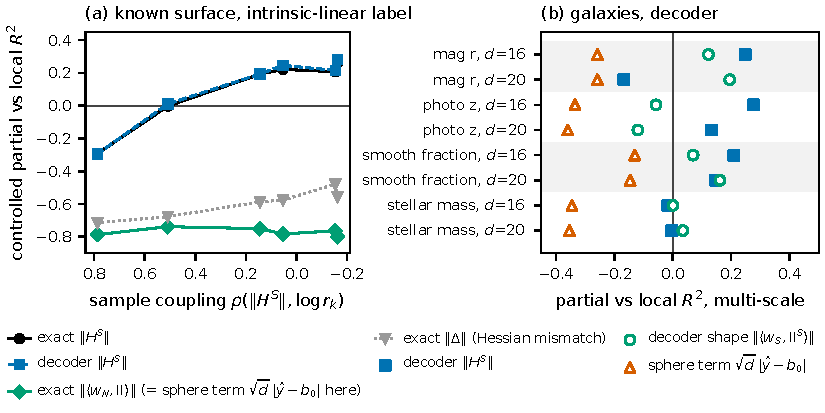
\includegraphics[width=0.85\textwidth]{figures/figF_mean_curvature.pdf}
\caption{(a) Known surface, linear label, exact geometry: three-control partial vs local $R^2$ as the density--curvature coupling is set by construction ($\gamma$ from $-1$ to $1$). (b) Galaxies, 512 anchors, $k=2{,}048$, multi-scale control: the decoder's $\norm{\Htan}$ (filled squares), shape term (open circles), sphere term (open triangles).}
\label{fig:meancurv}
\end{figure}
\end{document}
